\documentclass[10pt]{article}

% ============================================================
% PACKAGES (same constraint as the main guide: no tcolorbox / mdframed /
%  enumitem / titlesec on this machine — everything hand-rolled with xcolor)
% ============================================================
\usepackage[T1]{fontenc}
\usepackage{amsmath,amssymb,amsthm,mathtools}
\usepackage{geometry}
\geometry{letterpaper,margin=0.8in}
\usepackage{xcolor}
\usepackage{tikz}
\usepackage{booktabs}
\usepackage{array}
\usepackage{longtable}
\usepackage{parskip}
\usepackage{fancyhdr}
\usepackage[colorlinks=true,linkcolor=linkblue,citecolor=linkblue,urlcolor=linkblue,
            bookmarksnumbered=true,pdfborder={0 0 0}]{hyperref}
\usepackage{bookmark}

\setlength{\parskip}{2pt}

% ============================================================
% COLORS
% ============================================================
\definecolor{linkblue}{RGB}{20,60,130}
\definecolor{defcol}{RGB}{20,80,160}
\definecolor{thmcol}{RGB}{20,120,90}
\definecolor{flagcol}{RGB}{170,30,30}
\definecolor{flagbg}{RGB}{253,235,235}
\definecolor{exmcol}{RGB}{110,60,150}
\definecolor{notecol}{RGB}{150,90,10}
\definecolor{excol}{RGB}{30,90,140}
\definecolor{examcol}{RGB}{50,50,50}

% ============================================================
% MATH SHORTCUTS
% ============================================================
\newcommand{\E}[1]{\mathrm{E}\left[#1\right]}
\newcommand{\Var}[1]{\mathrm{Var}\left[#1\right]}
\newcommand{\Cov}[1]{\mathrm{Cov}\left[#1\right]}
\renewcommand{\P}[1]{P\left[#1\right]}

% ============================================================
% CHEAT-ENTRY MACROS: Name --- Statement --- Example --- "Use it when / how"
% Rule-line based (no filled boxes) so every entry is page-break safe.
% ============================================================
\newcommand{\cheat}[4]{%
  \par\vspace{6pt}\noindent{\color{thmcol}\rule{\linewidth}{1pt}}\par\vspace{2pt}
  \noindent\textbf{\color{thmcol}#1}\par\smallskip\noindent
  #2\par\smallskip
  \noindent{\small\color{excol}\textbf{Example:}} \small #3\par\smallskip
  \noindent{\small\color{notecol}\textbf{Use it when / how:}} \small #4\par
}

\newcommand{\cheatdef}[4]{%
  \par\vspace{6pt}\noindent{\color{defcol}\rule{\linewidth}{1pt}}\par\vspace{2pt}
  \noindent\textbf{\color{defcol}#1}\par\smallskip\noindent
  #2\par\smallskip
  \noindent{\small\color{excol}\textbf{Example:}} \small #3\par\smallskip
  \noindent{\small\color{notecol}\textbf{Use it when / how:}} \small #4\par
}

\newcommand{\cheatflag}[4]{%
  \par\vspace{7pt}\noindent{\color{flagcol}\rule{\linewidth}{1.3pt}}\par\vspace{1pt}
  \noindent{\color{flagcol}\rule{\linewidth}{0.4pt}}\par\vspace{2pt}
  \noindent\textbf{\color{flagcol}$\bigstar$ #1 $\bigstar$ \; [PROFESSOR-FLAGGED]}\par\smallskip\noindent
  #2\par\smallskip
  \noindent{\small\color{excol}\textbf{Example:}} \small #3\par\smallskip
  \noindent{\small\color{notecol}\textbf{Use it when / how:}} \small #4\par
  \vspace{1pt}\noindent{\color{flagcol}\rule{\linewidth}{0.4pt}}\par
}

% Exam problem box: Title --- Theorems Used --- full solution
\newcommand{\exambox}[3]{%
  \par\vspace{7pt}\noindent{\color{examcol}\rule{\linewidth}{1.1pt}}\par\vspace{2pt}
  \noindent\textbf{\color{examcol}#1}\par\smallskip
  \noindent{\small\color{notecol}\textbf{Theorems/tools used:}} \small #2\par\smallskip\noindent
  #3\par
}

\newcommand{\finalline}[1]{\par\vspace{4pt}\noindent{\color{#1}\rule{\linewidth}{1pt}}\par\vspace{4pt}}

% ============================================================
\pagestyle{fancy}
\fancyhf{}
\fancyhead[L]{\footnotesize\itshape Probability \& Stochastic Processes --- Theorem Cheat Sheet}
\fancyhead[R]{\footnotesize\itshape \leftmark}
\fancyfoot[C]{\thepage}
\renewcommand{\headrulewidth}{0.4pt}
\setlength{\headheight}{14pt}

\setcounter{tocdepth}{2}
\setcounter{secnumdepth}{2}
\tolerance=1400
\emergencystretch=3em
\hbadness=3000

\title{}
\date{}

\begin{document}
\thispagestyle{empty}
\begin{center}
{\Huge\bfseries Probability \& Stochastic Processes}\\[8pt]
{\LARGE Theorem Cheat Sheet}\\[4pt]
{\large\itshape Every Named Theorem, Definition, Worked Example \& When/How to Use It}\\[18pt]
{\normalsize Chapters 4 (\S4.2--4.3, 4.6--4.7) $\cdot$ 5 (\S5.7--5.9) $\cdot$ 6 (\S6.2--6.3) $\cdot$ 13 (\S13.6--13.11)}\\[4pt]
{\normalsize Plus every problem from Exam 1 and Exam 2, fully solved}
\end{center}

\vspace{10pt}
\noindent\fcolorbox{flagcol}{flagbg}{\parbox{\dimexpr\linewidth-2\fboxsep-2\fboxrule}{\centering
\textbf{\color{flagcol}How to read this sheet.} Every entry gives the exact textbook
number/name, the formula, a short \emph{worked numeric example}, and a note on \emph{when
you'd reach for it on an exam and how to apply it}. Entries the professor personally flagged
(Theorem 13.10, 13.11, 13.12, Example 13.22, and the bivariate Gaussian PDF) are marked
$\bigstar$ in red double-ruled boxes --- know these cold. Part~\ref{part:exams} at the end
solves every Exam 1 and Exam 2 problem, tagged with the exact theorems used above. This is a
companion to the full \textit{Final\_Exam\_Guide.pdf}, which has complete proofs as well.}}

\vspace{6pt}
\tableofcontents

\clearpage
% ================================================================
\section{Chapter 4 --- CDF, PDF, Gaussian RVs, Delta Functions}

\subsection{CDF and PDF Foundations (\S4.2--4.3)}

\cheatdef{Definition 4.1 --- Cumulative Distribution Function}{
$F_X(x) = \P{X\le x}$.
}{
Pointer spun on a 1-meter circle, $X\in[0,1)$ uniform: $F_X(x)=0$ for $x<0$, $F_X(x)=x$ for
$0\le x<1$, $F_X(x)=1$ for $x\ge1$.
}{
The universal probability model --- works for discrete, continuous, or mixed $X$. Reach for
this first whenever a problem defines a random variable in terms of ``the probability that
$X$ is at most $x$,'' or when you need $\P{a<X\le b}$.
}

\cheat{Theorem 4.1 --- Basic CDF Properties}{
$F_X(-\infty)=0$, $F_X(\infty)=1$, $\P{x_1<X\le x_2}=F_X(x_2)-F_X(x_1)$.
}{
For the pointer above, $\P{1/4<X\le3/4}=F_X(3/4)-F_X(1/4)=3/4-1/4=1/2$.
}{
Use property (c) any time you're asked for an interval probability and you already have (or
can derive) $F_X$. Use (a)/(b) as a sanity check on any CDF you derive --- if it doesn't go
from 0 to 1, you made an error.
}

\cheatdef{Definition 4.3 --- Probability Density Function}{
$f_X(x) = dF_X(x)/dx$.
}{
Differentiating $F_X(x)=x$ on $(0,1)$ gives $f_X(x)=1$ on $(0,1)$, $0$ elsewhere --- the
uniform PDF.
}{
Differentiate a CDF to get the PDF; conversely integrate a PDF to get the CDF (Theorem 4.2).
This is the two-way bridge you use constantly in Chapter 6 problems.
}

\cheat{Theorem 4.2 --- PDF Properties}{
$f_X(x)\ge0$; $F_X(x)=\int_{-\infty}^x f_X(u)\,du$; $\int_{-\infty}^{\infty}f_X(x)\,dx=1$.
}{
Given $f_X(x)=c(1-x^2)$ on $[-1,1]$ (Exam 1, Problem 4), normalization forces
$c\int_{-1}^1(1-x^2)dx=\tfrac43c=1\Rightarrow c=\tfrac34$.
}{
The normalization property ($\int f_X=1$) is exactly how you solve ``find the constant $c$/$A$''
problems --- set the total integral (or sum, for PMFs) equal to 1 and solve.
}

\cheat{Theorem 4.3 --- Interval Probability from the PDF}{
$\P{x_1<X\le x_2}=\int_{x_1}^{x_2}f_X(x)\,dx$.
}{
With $f_X(x)=1$ on $(0,1)$: $\P{1/4<X<3/4}=\int_{1/4}^{3/4}1\,dx=1/2$.
}{
Whenever you have $f_X$ (not yet $F_X$) and need a probability over a range, integrate
directly instead of first finding the full CDF --- faster when you only need one interval.
}

\cheatdef{Definition 4.4 --- Expected Value}{
$\E{X}=\int_{-\infty}^{\infty}xf_X(x)\,dx$.
}{
For $f_X(x)=1$ on $(0,1)$: $\E{X}=\int_0^1x\,dx=1/2$ meter --- the average pointer position.
}{
The ``average value'' of $X$. Always pair with Theorem 4.5(c) to get variance --- never
integrate $(x-\mu)^2f_X(x)$ directly if you can avoid it.
}

\cheat{Theorem 4.4 --- Law of the Unconscious Statistician (LOTUS)}{
$\E{g(X)}=\int_{-\infty}^{\infty}g(x)f_X(x)\,dx$.
}{
For $f_X(x)=1$ on $(0,1)$: $\E{X^2}=\int_0^1x^2\,dx=1/3$, obtained directly without ever
finding the PDF of $X^2$.
}{
\textbf{The single biggest time-saver in the course.} Use this whenever a question asks
only for $\E{g(X)}$ (e.g.\ $\E{X^2}$, $\E{e^X}$) --- you never need to derive the PDF of
$g(X)$ first. Only derive the full PDF of $W=g(X)$ (Chapter 6 machinery) if the question asks
for the whole distribution of $W$, not just its mean.
}

\cheat{Theorem 4.5 --- Linearity and Variance Identities}{
$\E{X-\mu_X}=0$; $\quad\E{aX+b}=a\E{X}+b$; $\quad\Var{X}=\E{X^2}-\mu_X^2$; $\quad\Var{aX+b}=a^2\Var{X}$.
}{
Continuing the pointer: $\E{X}=1/2$, $\E{X^2}=1/3\Rightarrow\Var{X}=1/3-1/4=1/12$.
}{
(c) is how \emph{every} variance computation is actually done on this exam: find $\E{X^2}$
and $\E{X}$ separately, then subtract the square. (b)/(d) let you rescale a random variable's
mean/variance instantly without re-deriving anything.
}

\subsection{Standard Continuous Families --- Mean and Variance for Each (\S4.5)}

\cheat{Definition 4.5 \& Theorem 4.6 --- Uniform$(a,b)$: PDF, CDF, $\E{},\Var{}$}{
$f_X(x)=\dfrac{1}{b-a}$ on $(a,b)$; $\ F_X(x)=\dfrac{x-a}{b-a}$ on $[a,b)$; $\quad
\E{X}=\dfrac{a+b}{2}$, $\quad\Var{X}=\dfrac{(b-a)^2}{12}$.
}{
Modem phase $\Theta\sim$Uniform$(0,2\pi)$: $\E{\Theta}=\pi$ rad,
$\Var{\Theta}=(2\pi)^2/12=\pi^2/3$ --- read straight off the formulas, no integration needed.
}{
Recognize ``uniform on $(a,b)$'' immediately and pull $\E{},\Var{}$ from the boxed formulas ---
never re-derive them by integrating $x/(b-a)$ from scratch.
}

\cheat{Definition 4.6 \& Theorem 4.8 --- Exponential$(\lambda)$: PDF, CDF, $\E{},\Var{}$}{
$f_X(x)=\lambda e^{-\lambda x}$, $x\ge0$; $\ F_X(x)=1-e^{-\lambda x}$; $\quad
\E{X}=\dfrac1\lambda$, $\quad\Var{X}=\dfrac1{\lambda^2}$.
}{
Call duration $T$ with $F_T(t)=1-e^{-t/3}\Rightarrow\lambda=1/3\Rightarrow\E{T}=3$ min,
$\Var{T}=9$ min$^2$, $\sigma_T=3$ min.
}{
Recognize $F_X(x)=1-e^{-\lambda x}$ (or $f_X=\lambda e^{-\lambda x}$) instantly as exponential
and read off the rate $\lambda$ --- this is the standard ``waiting time'' / ``arrival gap''
model.
}

\cheat{Definition 4.7 \& Theorem 4.10 --- Erlang$(n,\lambda)$: PDF, $\E{},\Var{}$}{
$f_X(x)=\dfrac{\lambda^nx^{n-1}e^{-\lambda x}}{(n-1)!}$, $x\ge0$; $\quad
\E{X}=\dfrac{n}{\lambda}$, $\quad\Var{X}=\dfrac{n}{\lambda^2}$.
}{
Sum of $n=4$ iid Exponential$(\lambda=2)$ waiting times is Erlang$(4,2)$: $\E{X}=4/2=2$,
$\Var{X}=4/4=1$ --- Erlang$(1,\lambda)$ reduces to plain Exponential$(\lambda)$.
}{
Recognize a sum of $n$ iid exponential$(\lambda)$ random variables (e.g.\ ``time until the
$n$th arrival'') as Erlang$(n,\lambda)$ and read $\E{},\Var{}$ directly --- no convolution
needed.
}

\cheat{Theorems 4.7, 4.9, 4.11 --- Bridges to Discrete Families}{
If $X\sim$Uniform$(a,b)$ (integer $a,b$), $K=\lceil X\rceil$ is discrete-uniform$(a{+}1,b)$
(Thm 4.7). If $X\sim$Exponential$(\lambda)$, $K=\lceil X\rceil$ is geometric$(p)$ with
$p=1-e^{-\lambda}$ (Thm 4.9). If $X\sim$Erlang$(n,\lambda)$,
$F_X(x)=\P{\text{Poisson}(\lambda x)\ge n}$ (Thm 4.11).
}{
$T\sim$Exponential$(1/3)$ (minutes): rounding \emph{up} to the next full minute,
$K=\lceil T\rceil$ is geometric$(p)$ with $p=1-e^{-1/3}\approx0.284$, so
$\E{K}=1/p\approx3.53$ minutes billed --- more than $\E{T}=3$, since rounding up always costs
extra.
}{
Use these whenever a continuous waiting-time model gets \emph{rounded/discretized} (e.g.\
billing by the minute) or whenever you need to relate an Erlang CDF to a Poisson probability
--- they are the formal link between the continuous-time family (Ch.\ 4) and the
discrete-time/counting family (Ch.\ 3, and later the Poisson process in Ch.\ 13).
}

\subsection{Gaussian Random Variables (\S4.6)}

\cheatdef{Definition 4.8 --- Gaussian Random Variable}{
$f_X(x)=\dfrac{1}{\sqrt{2\pi}\sigma}e^{-(x-\mu)^2/2\sigma^2}$, written $X\sim N[\mu,\sigma^2]$.
}{
A test score is $X\sim N[61,100]$ (i.e.\ $\mu=61$, $\sigma=10$).
}{
Recognize this bell-curve form immediately whenever a problem says ``Gaussian,'' ``normal,''
or gives you this exact exponential form (including inside a joint PDF --- see \S5.9 below).
}

\cheat{Theorem 4.12 --- Gaussian Mean and Variance}{
$\E{X}=\mu$, $\quad\Var{X}=\sigma^2$.
}{
$X\sim N[61,100]$: read off instantly $\E{X}=61$, $\Var{X}=100$ ($\sigma=10$).
}{
Read the parameters straight off the notation $N[\mu,\sigma^2]$ --- no integration needed.
}

\cheat{Theorem 4.13 --- Linear Transform of a Gaussian}{
If $X\sim N[\mu,\sigma^2]$, then $Y=aX+b\sim N[a\mu+b,\ a^2\sigma^2]$.
}{
If $Z\sim N[0,1]$ and $X=10Z+61$, then $X\sim N[61,100]$ --- the standardizing transform run
in reverse.
}{
Use whenever a problem defines a new r.v.\ as an affine function of a Gaussian (e.g.\
rescaled voltage, shifted temperature) --- you get the new distribution instantly without
re-deriving a PDF.
}

\cheatdef{Definitions 4.9 \& 4.10 --- Standard Normal $Z$ and Its CDF $\Phi$}{
$Z$ is the Gaussian$(0,1)$ r.v.; $\quad\Phi(z)=\dfrac{1}{\sqrt{2\pi}}\displaystyle\int_{-\infty}^{z}e^{-u^2/2}\,du$.
}{
By Theorem 4.13, standardizing $X\sim N[\mu,\sigma^2]$ via $Z=(X-\mu)/\sigma$ always produces
exactly this $Z\sim N[0,1]$ --- which is why a single table of $\Phi$ values covers every
Gaussian random variable.
}{
Every Gaussian probability calculation bottoms out in a table lookup of $\Phi(z)$ for this one
specific $Z$ --- Theorem 4.14 (next) is simply the recipe for getting there from any
$N[\mu,\sigma^2]$.
}

\cheat{Theorem 4.14 --- Gaussian CDF via $\Phi$}{
$F_X(x)=\Phi\!\left(\dfrac{x-\mu}{\sigma}\right)$, $\quad
\P{a<X\le b}=\Phi\!\left(\dfrac{b-\mu}{\sigma}\right)-\Phi\!\left(\dfrac{a-\mu}{\sigma}\right)$.
}{
$X\sim N[61,100]$: $\P{51<X<71}=\Phi(1)-\Phi(-1)=2\Phi(1)-1=2(0.8413)-1=0.683$.
}{
\textbf{The standard tool for every ``find the probability'' Gaussian question.} Standardize
to $z=(x-\mu)/\sigma$, then look up $\Phi(z)$ in the table.
}

\cheat{Theorem 4.15 --- Symmetry of $\Phi$}{
$\Phi(-z)=1-\Phi(z)$.
}{
$\P{X<46}=\Phi\!\left(\tfrac{46-61}{10}\right)=\Phi(-1.5)=1-\Phi(1.5)=1-0.9332=0.067$.
}{
Use whenever your $z$-score comes out negative but your table only lists $\Phi$ for positive
$z$.
}

\cheatdef{Definition 4.11 --- $Q$-function (complementary CDF)}{
$Q(z)=1-\Phi(z)=\P{Z>z}$.
}{
Exam 1, Problem 5: bit-error probability with SNR$=4$ is $Q(2)=1-\Phi(2)=1-0.97725=0.02275$.
}{
\textbf{Always the right tool for ``rare event'' / tail / bit-error-rate questions} (e.g.\
$\P{\text{noise exceeds threshold}}$) --- these are phrased in terms of $Q$, not $\Phi$,
because $Q$ resolves the small-tail-probability precision that $\Phi$ loses near 1.
}

\subsection{Delta Functions \& Mixed Random Variables (\S4.7)}

\cheatdef{Definition 4.12 --- Unit Impulse (Delta) Function}{
$\delta(x)=\lim_{\epsilon\to0}d_\epsilon(x)$, with $\int_{-\infty}^{\infty}\delta(x)\,dx=1$.
}{
$Y\in\{1,2,3\}$ each with probability $1/3$ has PDF $f_Y(y)=\tfrac13\delta(y-1)+\tfrac13\delta(y-2)+\tfrac13\delta(y-3)$.
}{
Whenever a random variable has a point mass (discrete part) embedded in an otherwise
continuous PDF, that point mass is represented as $p\,\delta(x-x_0)$ in $f_X(x)$.
}

\cheat{Theorem 4.16 --- Sifting Property}{
$\displaystyle\int_{-\infty}^{\infty}g(x)\,\delta(x-x_0)\,dx=g(x_0)$.
}{
$\E{Y}=\int y\left[\tfrac13\delta(y-1)+\tfrac13\delta(y-2)+\tfrac13\delta(y-3)\right]dy
=\tfrac13(1)+\tfrac13(2)+\tfrac13(3)=2$.
}{
Use this to evaluate $\E{X}$, $\E{g(X)}$, or any integral once impulses appear in the PDF ---
the impulse just ``picks out'' the integrand's value at $x_0$, turning the integral into
plain evaluation.
}

\cheat{Theorem 4.17 --- Step/Delta Relationship}{
$\int_{-\infty}^{x}\delta(v)\,dv=u(x)$, equivalently $\delta(x)=du(x)/dx$.
}{
The CDF jump of $1/3$ at $y=1$ (from the example above) corresponds to the impulse term
$\tfrac13\delta(y-1)$ in $f_Y(y)$.
}{
Use to convert between a discrete RV's PMF-based CDF (a staircase built from $u(x-x_i)$) and
its impulse-based PDF ($\sum P_X(x_i)\delta(x-x_i)$), and vice versa.
}

\cheat{Theorem 4.18 --- Four Equivalent Ways to State ``a Point Has Probability $q$''}{
For any random variable $X$, these are equivalent: (a) $\P{X=x_0}=q$; (b) $P_X(x_0)=q$;
(c) $F_X(x_0^+)-F_X(x_0^-)=q$; (d) $f_X(x_0)=q\,\delta(0)$.
}{
Exam 1, Problem 1: the impulse $\tfrac18\delta(x+2)$ in $f_X$ (form (d)) is exactly the same
fact as the CDF jump $F_X(-2)-F_X(-2^-)=\tfrac18$ (form (c)) and $\P{X=-2}=\tfrac18$ (form (a)).
}{
Use whenever a problem switches between describing a point mass as ``probability $q$ at
$x_0$,'' ``a jump of size $q$ in $F_X$,'' or ``an impulse $q\,\delta(x-x_0)$ in $f_X$'' ---
they are the same information in three notations; pick whichever is easiest for the step
you're on.
}

\cheatdef{Definition 4.14 --- Mixed Random Variable}{
$X$ is mixed iff $f_X(x)$ contains \emph{both} impulses and nonzero finite (continuous)
values.
}{
Phone call duration: $1/3$ chance the call never connects ($Y=0$), else uniform$(0,3)$ minutes:
$f_Y(y)=\tfrac13\delta(y)+\tfrac29$ on $[0,3)$, giving $\E{Y}=1$ minute.
}{
Recognize a mixed RV whenever a problem describes ``with probability $p$ nothing happens
(point mass), otherwise $X$ is continuous on some range'' --- write $f_X$ as (impulse term)
$+$ (continuous term), find the impulse weight from the point-mass probability, and the
continuous piece from the conditional continuous density times its probability.
}

\clearpage
% ================================================================
\section{Chapter 5 --- Multiple Random Variables}

\subsection{Marginal PMF/PDF --- Foundational (\S5.3, \S5.5)}

\cheatdef{Marginal PMF and Marginal PDF}{
$P_X(x)=\displaystyle\sum_{y\in S_Y}P_{X,Y}(x,y)$; \qquad
$f_X(x)=\displaystyle\int_{-\infty}^{\infty}f_{X,Y}(x,y)\,dy$ (and symmetrically for
$P_Y(y)$, $f_Y(y)$).
}{
$f_{X,Y}(x,y)=\tfrac{x+y}{3}$ on $0\le x\le1,\,0\le y\le2$ (Exam 1, Problem 2):
$f_X(x)=\int_0^2\tfrac{x+y}3\,dy=\tfrac{2x+2}3$ on $0\le x\le1$.
}{
\textbf{The mandatory first step whenever a problem gives you a joint model but asks about
only one variable} ($\E{X}$, $\Var{X}$, $P[X\in A]$, etc.) --- sum out (discrete) or integrate
out (continuous) the \emph{other} variable, then treat the result as an ordinary
single-variable PMF/PDF and apply the Chapter 3/4 tools you already know.
}

\subsection{Expected Value of a Function of Two RVs (\S5.7)}

\cheat{Theorem 5.9 --- $\E{g(X,Y)}$}{
Discrete: $\sum_x\sum_y g(x,y)P_{X,Y}(x,y)$. \quad Continuous: $\iint g(x,y)f_{X,Y}(x,y)\,dx\,dy$.
}{
Transmission time $T=8L/(1000R)$ with independent speed $R$ and length $L$: $\E{T}=1.652$
seconds (Example 5.15) --- note this is \emph{not} equal to $g(\E R,\E L)=1.475$ seconds.
}{
The two-variable version of LOTUS (Theorem 4.4) --- use whenever you need $\E{g(X,Y)}$ for
\emph{any} function $g$ (not just $X+Y$ or $XY$) and you have the joint model.
}

\cheat{Theorem 5.10 --- Linearity of Expectation (General Case)}{
$\E{a_1g_1(X,Y)+\cdots+a_ng_n(X,Y)} = a_1\E{g_1(X,Y)}+\cdots+a_n\E{g_n(X,Y)}$.
}{
$\E{3X^2-2XY+5} = 3\E{X^2}-2\E{XY}+5$ --- each piece computed separately via Theorem 5.9, then
recombined with its coefficient.
}{
Use whenever the quantity you need is a \emph{linear combination} of several functions of
$X,Y$ (not just one $g$) --- split it into pieces, apply Theorem 5.9 to each piece
independently, and recombine. Theorem 5.11 below is the special case $g_1=X,g_2=Y,a_1=a_2=1$.
}

\cheat{Theorem 5.11 --- Expected Value of a Sum}{
$\E{X+Y}=\E{X}+\E{Y}$.
}{
Exam 2, Problem 1 ($f_{X,Y}=4xy$ on the unit square): $\E{X}=\E{Y}=2/3\Rightarrow\E{X+Y}=4/3$.
}{
\textbf{Always true, even if $X,Y$ are dependent}, and needs only the marginals. Use this
first before reaching for the joint PDF --- it's very often all you need for an ``$\E{X+Y}$''
question.
}

\cheat{Theorem 5.12 --- Variance of a Sum}{
$\Var{X+Y}=\Var{X}+\Var{Y}+2\Cov{X,Y}$.
}{
Same problem: $\Var{X}=\Var{Y}=1/18$, $\Cov{X,Y}=0\Rightarrow\Var{X+Y}=1/18+1/18+0=1/9$.
}{
Unlike $\E{X+Y}$, this \emph{needs} the joint model (through the covariance term) unless you
already know $X,Y$ are independent (then $\Cov{X,Y}=0$ and it reduces to just
$\Var{X}+\Var{Y}$). This contrast is a favorite exam trap --- know it cold.
}

\subsection{Covariance, Correlation, Independence (\S5.8)}

\cheatdef{Definition 5.5 --- Covariance}{
$\Cov{X,Y}=\E{(X-\mu_X)(Y-\mu_Y)}$.
}{
For $f_{X,Y}=4xy$ on the unit square: $\E{XY}=4/9$, $\E{X}\E{Y}=(2/3)^2=4/9\Rightarrow
\Cov{X,Y}=0$.
}{
Never compute this by direct integration if you can avoid it --- use Theorem 5.16(a) instead
($\Cov{X,Y}=\E{XY}-\E{X}\E{Y}$), which is how every real exam solution does it.
}

\cheatdef{Definition 5.6 --- Correlation Coefficient}{
$\rho_{X,Y}=\Cov{X,Y}/(\sigma_X\sigma_Y)$.
}{
Exam 2, Problem 2 ($f_{X,Y}=ce^{-(2x^2-4xy+4y^2)}$): matching to the bivariate Gaussian form
gives $\rho_{X,Y}=1/\sqrt2$.
}{
The unit-free measure of linear relationship. Compute $\Cov{X,Y}$, $\sigma_X$, $\sigma_Y$
separately, then divide. Always check your answer satisfies $-1\le\rho_{X,Y}\le1$
(Theorem 5.14) --- if not, you have an arithmetic error.
}

\cheat{Theorem 5.13 --- $\rho$ and $\Cov{}$ Under Linear Rescaling}{
If $\hat X=aX+b$, $\hat Y=cY+d$: $\quad\rho_{\hat X,\hat Y}=\rho_{X,Y}$ (unchanged!), \qquad
$\Cov{\hat X,\hat Y}=ac\,\Cov{X,Y}$.
}{
Height/weight in cm/kg vs.\ inches/lbs: $\Cov{}$ changes by the unit-conversion factors, but
$\rho_{X,Y}$ (e.g.\ $\approx0.7$) is exactly the same number in either unit system.
}{
Use whenever a problem changes units or rescales one or both variables --- $\rho_{X,Y}$ is
\emph{invariant} (that's the whole point of normalizing by $\sigma_X\sigma_Y$), while
$\Cov{X,Y}$ scales by the product $ac$ of the two scale factors.
}

\cheat{Theorem 5.14 --- Correlation Coefficient Is Bounded}{
$-1\le\rho_{X,Y}\le1$.
}{
$\rho_{X,Y}=1/\sqrt2\approx0.707$ from the example above satisfies $|0.707|\le1$ --- passes
the sanity check.
}{
Use as an automatic sanity check on every $\rho$ you compute.
}

\cheat{Theorem 5.15 --- Correlation of a Perfect Linear Relationship}{
If $Y=aX+b$: $\rho_{X,Y}=-1$ ($a<0$), $0$ ($a=0$), $1$ ($a>0$).
}{
If gain $Y$ (dB) $=-1\times$attenuation $X$ (dB) $+\,b$, then instantly $\rho_{X,Y}=-1$.
}{
Use to instantly answer ``what is $\rho_{X,Y}$'' questions where $Y$ is given as an exact
linear function of $X$ --- no computation needed.
}

\cheatdef{Definition 5.7 --- Correlation}{
$r_{X,Y}=\E{XY}$.
}{
Exam 2, Problem 5 (joint PMF $P_{X,Y}(x,y)=1/(4x)$ for $1\le y\le x\le4$): $r_{X,Y}=\E{XY}=5$.
}{
Compute this first (via Theorem 5.9 with $g(x,y)=xy$) --- it feeds directly into
Theorem 5.16(a) for covariance.
}

\cheat{Theorem 5.16 --- The Master Covariance/Variance Identities}{
(a) $\Cov{X,Y}=r_{X,Y}-\mu_X\mu_Y$. \quad
(b) $\Var{X+Y}=\Var{X}+\Var{Y}+2\Cov{X,Y}$. \quad
(c) If $X=Y$: $\Cov{X,Y}=\Var{X}$, $r_{X,Y}=\E{X^2}$.
}{
Continuing Exam 2 Problem 5: $r_{X,Y}=5$, $\E{X}=5/2$, $\E{Y}=7/4\Rightarrow
\Cov{X,Y}=5-(5/2)(7/4)=10/16$.
}{
\textbf{This is the workhorse of every Chapter 5 exam problem.} Standard solution path: find
$\E{X}$, $\E{Y}$, $\E{XY}$ (via Theorem 5.9) $\to$ get $\Cov{X,Y}$ via (a) $\to$ get
$\rho_{X,Y}$ by dividing by $\sigma_X\sigma_Y$ $\to$ get $\Var{X+Y}$ via (b) if asked.
}

\cheatdef{Definition 5.8/5.9 --- Orthogonal vs.\ Uncorrelated}{
Orthogonal: $r_{X,Y}=0$. \quad Uncorrelated: $\Cov{X,Y}=0$.
}{
Exam 2, Problem 4 ($f_{X,Y}=1/2$ on $-1\le x\le y\le1$): $r_{X,Y}=\E{XY}=0$, so $X,Y$ are
orthogonal; since also $\E{X}=0$ here, they're uncorrelated too.
}{
Watch the exact wording of a question --- ``orthogonal'' asks about $\E{XY}$, ``uncorrelated''
asks about $\Cov{X,Y}=\E{XY}-\E{X}\E{Y}$. They coincide only when $\E{X}=0$ or $\E{Y}=0$.
}

\cheat{Theorem 5.17 --- Independence $\Rightarrow$ Uncorrelated (Not Conversely)}{
Independent $X,Y$ $\Rightarrow$ $\E{g(X)h(Y)}=\E{g(X)}\E{h(Y)}$, \ $r_{X,Y}=\E{X}\E{Y}$,
\ $\Cov{X,Y}=\rho_{X,Y}=0$, \ $\Var{X+Y}=\Var{X}+\Var{Y}$.
}{
Signal $X\sim N[0,\sigma_X^2]$ and independent noise $Z\sim N[0,\sigma_Z^2]$: $\Cov{X,Z}=0$
and $\Var{X+Z}=\sigma_X^2+\sigma_Z^2$ follow immediately from independence.
}{
Use the forward direction freely once independence is given/shown. \textbf{Never use the
converse} --- uncorrelated does \textbf{NOT} imply independent --- unless the pair is
bivariate Gaussian (Theorem 5.20), a very common exam trap otherwise.
}

\subsection{Bivariate Gaussian Random Variables (\S5.9)}

\cheatflag{Definition 5.10 --- The Bivariate Gaussian PDF}{
\[
f_{X,Y}(x,y)=\frac{1}{2\pi\sigma_X\sigma_Y\sqrt{1-\rho^2}}
\exp\!\left[-\frac{\left(\frac{x-\mu_X}{\sigma_X}\right)^2-\frac{2\rho(x-\mu_X)(y-\mu_Y)}{\sigma_X\sigma_Y}+\left(\frac{y-\mu_Y}{\sigma_Y}\right)^2}{2(1-\rho^2)}\right].
\]
}{
Exam 2, Problem 2: matching $ce^{-(2x^2-4xy+4y^2)}$ term-by-term to this exponent gives
$\sigma_X=1/\sqrt2$, $\sigma_Y=1/2$, $\rho=1/\sqrt2$, and then
$c=1/(2\pi\sigma_X\sigma_Y\sqrt{1-\rho^2})=2/\pi$.
}{
\textbf{Memorize this exact formula.} When you're handed a joint PDF of the form
$c\,e^{-(\text{quadratic in }x,y)}$, match the quadratic's coefficients term-by-term against
the exponent above to read off $\sigma_X,\sigma_Y,\rho$ (and hence $c$). It has 5 parameters:
$\mu_X,\mu_Y,\sigma_X,\sigma_Y,\rho_{X,Y}$.
}

\cheat{Theorem 5.18 --- Marginals of a Bivariate Gaussian}{
If $X,Y$ are bivariate Gaussian, $X\sim N[\mu_X,\sigma_X^2]$ and $Y\sim N[\mu_Y,\sigma_Y^2]$.
}{
From Exam 2 Problem 2: the marginal of $X$ alone is $N[0,1/2]$, regardless of $\rho$.
}{
Use whenever you need just the marginal distribution of $X$ or $Y$ from a bivariate Gaussian
joint PDF --- $\rho$ drops out entirely for a single-variable marginal.
}

\cheat{Theorem 5.19 --- $\rho$ Really Is the Correlation Coefficient}{
The parameter $\rho$ in Definition 5.10 equals $\rho_{X,Y}$ as defined in Definition 5.6.
}{
In Exam 2 Problem 2, once you match coefficients and get $\rho=1/\sqrt2$, that \emph{is}
$\Cov{X,Y}/(\sigma_X\sigma_Y)$ --- no separate computation needed.
}{
Justifies reading $\rho$ directly off the bivariate Gaussian formula instead of computing
$\Cov{X,Y}/(\sigma_X\sigma_Y)$ from scratch.
}

\cheatflag{Theorem 5.20 --- Uncorrelated $\Leftrightarrow$ Independent (Bivariate Gaussian Only)}{
Bivariate Gaussian $X,Y$: uncorrelated $\iff$ independent.
}{
Exam 2, Problem 2: since $\rho=1/\sqrt2\ne0$, $X,Y$ are \textbf{dependent} --- this theorem is
exactly why $\rho\ne0$ alone is enough to conclude dependence for a bivariate Gaussian pair.
}{
\textbf{The one and only exception to Theorem 5.17's one-way arrow.} Use this whenever the
problem states or implies $X,Y$ are jointly Gaussian --- then (and only then) $\rho=0$ lets
you conclude independence.
}

\cheat{Theorem 5.21 --- Linear Combinations of Jointly Gaussian Variables}{
If $X,Y$ bivariate Gaussian, $W_1=a_1X+b_1Y$, $W_2=a_2X+b_2Y$ are also bivariate Gaussian, with
means/variances/covariance given by the usual bilinear formulas.
}{
$X\sim N[0,16]$, $Z\sim N[0,9]$ independent, $Y=X+Z$: $Y\sim N[0,25]$ and
$\rho_{X,Y}=\sqrt{(16/9)/(1+16/9)}=4/5$.
}{
Use whenever a problem defines new variables as linear combinations of jointly Gaussian
$X,Y$ (e.g.\ $Y=X+Z$ signal-plus-noise) --- you instantly know the result is Gaussian, so only
the mean/variance/covariance remain to compute.
}

\clearpage
% ================================================================
\section{Chapter 6 --- Functions of Random Variables}

\cheat{Theorem 6.1 --- PMF of a Function of Two Discrete Random Variables (\S6.1)}{
$P_W(w)=\displaystyle\sum_{(x,y):\,g(x,y)=w}P_{X,Y}(x,y)$.
}{
Newsletter cost $W=LX$ (length $\times$ per-page rate): $W=120$ arises from \emph{two}
different $(l,x)$ pairs, $(2,60)$ and $(3,40)$, so $P_W(120)=P_{L,X}(2,60)+P_{L,X}(3,40)$ ---
add the probabilities of every input pair that maps to the same output value.
}{
The discrete analog of the Chapter 6 method: whenever several $(x,y)$ pairs give the \emph{same}
$w=g(x,y)$, their probabilities \emph{add}. Always check whether a given output value has more
than one pre-image before writing down $P_W(w)$.
}

\cheat{The General Method (\S6.2)}{
To find $f_W(w)$ for $W=g(X)$: (1) find $F_W(w)=\P{g(X)\le w}$ by identifying which $x$
satisfy $g(x)\le w$; (2) differentiate, $f_W(w)=dF_W(w)/dw$.
}{
Pointer $X$ uniform$(0,1)$ meters, $W=100X$ cm: $F_W(w)=\P{X\le w/100}=F_X(w/100)=w/100$ on
$(0,100)\Rightarrow f_W(w)=1/100$, i.e.\ $W\sim$Uniform$(0,100)$.
}{
\textbf{Use this whenever you need the full distribution of a transformed random variable}
--- especially when $g$ is not monotonic (e.g.\ $Y=X^2$, $Y=cX^2$, any limiter/clipper). If
you only need $\E{g(X)}$, use LOTUS (Theorem 4.4) instead --- much faster.
}

\cheat{Theorem 6.2 --- Scaling: $W=aX,\ a>0$}{
$F_W(w)=F_X(w/a)$, \quad $f_W(w)=\frac1a f_X(w/a)$.
}{
$X$ triangular, $f_X(x)=2x$ on $(0,1)$; $W=aX\Rightarrow f_W(w)=\tfrac1a f_X(w/a)=2w/a^2$ on
$(0,a)$.
}{
Use for any pure rescaling of a random variable (unit conversions, gain factors).
}

\cheat{Theorem 6.3 --- Scaling Within Standard Families ($W=aX,\ a>0$)}{
Uniform$(b,c)\to$Uniform$(ab,ac)$; \ Exponential$(\lambda)\to$Exponential$(\lambda/a)$; \
Erlang$(n,\lambda)\to$Erlang$(n,\lambda/a)$; \ Gaussian$(\mu,\sigma)\to$Gaussian$(a\mu,a\sigma)$.
}{
$X\sim$Exponential$(\lambda=2)$, $W=3X$: by the table, $W\sim$Exponential$(2/3)$ ---
confirmed by Theorem 6.2: $f_W(w)=\tfrac13(2)e^{-2(w/3)}=\tfrac23e^{-(2/3)w}$, rate $2/3$.
}{
Whenever $W=aX$ and $X$ belongs to one of the four standard continuous families, skip
Theorem 6.2's derivation entirely and just read the new parameter off this table.
}

\cheat{Theorem 6.4 --- Shift: $W=X+b$}{
$F_W(w)=F_X(w-b)$, \quad $f_W(w)=f_X(w-b)$.
}{
$X\sim$Uniform$(0,1)$, $W=X-2$: $f_W(w)=f_X(w+2)=1$ on $(-2,-1)$ --- just the uniform density
slid left by 2.
}{
Combine with Theorem 6.2 for the general affine case $W=aX+b$: $f_W(w)=\frac1a
f_X\!\left(\frac{w-b}{a}\right)$.
}

\cheatflag{Squaring a Random Variable, e.g.\ $Y=cX^2$ (Example 6.4)}{
Since $Y$ can never be negative, ``$Y$ is at most $y$'' means ``$X$ is somewhere between
$-\sqrt{y/c}$ and $+\sqrt{y/c}$.'' So: rewrite the event that way, find its probability using
$X$'s own density, then differentiate at the end to get $Y$'s density.
}{
\textbf{Exam 2, Problem 3, worked in full:} $X$ is the current, Uniform$(-2,2)$; $Y=9X^2$ is
the power. \textit{Step 1:} since $X$ is between $-2$ and $2$, $Y=9X^2$ can only land between
$0$ and $36$. \textit{Step 2:} ``$Y\le y$'' means ``$-\sqrt{y/9}\le X\le\sqrt{y/9}$.'' Because
$X$ is uniform, that's just (length of that stretch)/(total length $4$) $=\sqrt y/6$ --- so
$F_Y(y)=\sqrt y/6$. \textit{Step 3:} take the derivative: $f_Y(y)=1/(12\sqrt y)$, for $y$
between $0$ and $36$.
}{
\textbf{This is the exact recipe for every ``power'' or ``energy'' problem} (``current $X$ is
uniform, power $Y=cX^2$, find the probability curve of $Y$'') --- it appeared almost word for
word on Exam 2. In plain terms: (1) figure out the smallest and largest values $Y$ could be,
using the smallest/largest values $X$ could be; (2) turn ``$Y\le y$'' into a statement about
$X$ being between two square-root bounds; (3) find that probability directly from $X$'s
density (watch out --- if those square-root bounds ever stick out past where $X$ is actually
allowed to be, stop them at $X$'s own edge instead); (4) differentiate to get $Y$'s density.
}

\cheat{Theorem 6.5 --- Inverse-CDF Method}{
If $U\sim$Uniform$(0,1)$ and $F$ is an invertible CDF, then $X=F^{-1}(U)$ has CDF $F$.
}{
Target Exponential(1): solve $u=1-e^{-x}\Rightarrow x=-\ln(1-u)$, so $X=-\ln(1-U)$ is
Exponential(1).
}{
Use to \emph{construct} a random variable with a target distribution from a Uniform(0,1)
generator (simulation-style questions). Fails for Gaussian (no closed-form inverse) and for
mixed random variables.
}

\cheatflag{A Meter That Can't Read Past a Certain Value (Examples 6.7--6.8, \S6.3)}{
Below the cutoff, nothing changes --- the density stays exactly what it was. At the cutoff
itself, every probability that ``would have gone higher'' piles up into one single spot,
sized to whatever was left over.
}{
\textbf{Exam 2, Problem 3(c), worked in full:} the power meter reads $W=Y$ normally, but shows
$16$ for anything $16$ or above. \textit{Step 1:} below $16$, $W$ behaves exactly like $Y$, so
$F_W(w)=F_Y(w)=\sqrt w/6$ there --- unchanged. \textit{Step 2:} right at $w=16$, the chance
that used to be spread out above $16$ (that's $1-F_Y(16)=1-4/6=1/3$) all lands in one pile
exactly at $16$. \textit{Result:} $f_W(w)=\tfrac{1}{12\sqrt w}$ for $w$ below $16$, plus one
extra pile of size $\tfrac13$ sitting exactly at $w=16$.
}{
\textbf{Use whenever a variable is described as ``capped,'' ``limited,'' or ``can't read
past'' some value} (a power meter that maxes out, a voltage clipper, etc.) --- this exact
setup appeared on Exam 2, Problem 3(c). The result always has this same two-part shape: an
ordinary curve below the cap, plus one single pile of leftover probability sitting right at
the cap.
}

\clearpage
% ================================================================
\section{Chapter 13 --- Stochastic Processes}

\subsection{Mean, Correlation, and the Stationarity Definitions (\S13.7--13.8)}

\cheatdef{Definition 13.11/13.12/13.13 --- Mean, Autocovariance, Autocorrelation}{
$\mu_X(t)=\E{X(t)}$; \quad $C_X(t,\tau)=\Cov{X(t),X(t+\tau)}$; \quad
$R_X(t,\tau)=\E{X(t)X(t+\tau)}$.
}{
Random-phase carrier $X(t)=A\cos(2\pi f_ct+\Theta)$, $\Theta\sim$Uniform$(0,2\pi)$ (Example
13.22): $\mu_X(t)=0$ for all $t$, and $R_X(t,\tau)=(A^2/2)\cos(2\pi f_c\tau)$.
}{
These three functions are the \emph{first} thing to compute for any named process. Note
$R_X(t,0)=\E{X^2(t)}$ is the process's instantaneous average power.
}

\cheat{Theorem 13.9 --- Autocovariance from Autocorrelation}{
$C_X(t,\tau)=R_X(t,\tau)-\mu_X(t)\mu_X(t+\tau)$.
}{
For the random-phase carrier (zero mean): $C_X(t,\tau)=R_X(t,\tau)-0=R_X(t,\tau)$ --- mean and
autocovariance coincide whenever $\mu_X=0$.
}{
Use to convert between the two whenever a problem gives you one and asks for the other ---
identical in spirit to $\Cov{X,Y}=\E{XY}-\E{X}\E{Y}$ (Theorem 5.16(a)), just evaluated at two
time instants.
}

\cheatdef{Definition 13.14 --- Stationary Process}{
Every joint PDF of $X(t_1),\dots,X(t_m)$ is unchanged under a common time shift $\tau$.
}{
White Gaussian noise (Definition 13.20) is stationary: it's WSS by construction, and
Theorem 13.15 (WSS $+$ Gaussian $\Rightarrow$ stationary) upgrades that to full stationarity
without checking every joint PDF by hand.
}{
The strict, hardest-to-verify definition --- in practice you almost always check the easier
WSS conditions (Definition 13.15) instead, since stationary $\Rightarrow$ WSS (Theorem 13.11).
}

\cheatflag{Theorem 13.10 --- Linear Transformations Preserve Stationarity}{
$X(t)$ stationary $\Rightarrow$ $Y(t)=aX(t)+b$ ($a>0$) is also stationary.
}{
If $X(t)$ is a stationary noise voltage and an amplifier outputs $Y(t)=5X(t)+2$, then $Y(t)$
is automatically stationary too --- no re-derivation needed.
}{
Use whenever a new process is defined as an affine function of a known stationary process ---
you get stationarity of $Y(t)$ for free, with no need to re-check every joint PDF.
}

\cheatflag{Theorem 13.11 --- Three Consequences of Stationarity}{
Stationary $X(t)$ $\Rightarrow$ (a) $\mu_X(t)=\mu_X$ (constant); (b) $R_X(t,\tau)=R_X(\tau)$
($\tau$ only); (c) $C_X(t,\tau)=R_X(\tau)-\mu_X^2=C_X(\tau)$.
}{
Random-phase carrier (Example 13.22): $\mu_X(t)=0$ for all $t$ (constant, satisfies (a)) and
$R_X(t,\tau)=(A^2/2)\cos(2\pi f_c\tau)$ depends on $\tau$ only (satisfies (b)).
}{
\textbf{This is your checklist for ``is this process stationary/WSS.''} Compute $\mu_X(t)$
and $R_X(t,\tau)$ directly from the process's definition, then check (a) and (b) in order ---
if either fails, the process is \emph{not} stationary (and, since stationary $\Rightarrow$
WSS, likely not WSS either).
}

\cheatflag{Example 13.22 --- The Random-Phase AM Carrier}{
$X(t)=A\cos(2\pi f_ct+\Theta)$, $\Theta\sim$Uniform$(0,2\pi)$: $\ \mu_X(t)=0$, \quad
$R_X(t,\tau)=\dfrac{A^2}{2}\cos(2\pi f_c\tau)=R_X(\tau)$.
}{
Worked in full: using $E[\cos(a+k\Theta)]=0$ for any fixed $a$, nonzero integer $k$, expand
$\cos A\cos B=\tfrac12[\cos(A-B)+\cos(A+B)]$ with $A-B=-2\pi f_c\tau$ constant --- the
$\cos(A+B)$ term (which contains $2\Theta$) averages to zero, leaving
$R_X(t,\tau)=\tfrac{A^2}2\cos2\pi f_c\tau$.
}{
\textbf{The professor's flagship worked example --- know the setup and result by heart.} Use
this exact template for \emph{any} ``random phase cosine/sinusoid'' process question ---
constant zero mean and $\tau$-only autocorrelation $\Rightarrow$ WSS (Example 13.23).
}

\subsection{Wide Sense Stationarity \& Ergodicity (\S13.9)}

\cheatdef{Definition 13.15 --- Wide Sense Stationary (WSS)}{
$\E{X(t)}=\mu_X$ (constant) and $R_X(t,\tau)=R_X(\tau)$ (depends on $\tau$ only).
}{
The random-phase carrier of Example 13.22 has $\mu_X=0$ (constant) and
$R_X(\tau)=(A^2/2)\cos2\pi f_c\tau$ ($\tau$-only) $\Rightarrow$ WSS (Example 13.23).
}{
\textbf{The practical, easy-to-check property you'll actually use on the exam} (weaker than
full stationarity, and every stationary process is automatically WSS by Theorem 13.11). Check
these two conditions directly from $\mu_X(t)$ and $R_X(t,\tau)$ --- don't bother with the full
joint-PDF definition unless explicitly asked for strict-sense stationarity.
}

\cheatflag{Theorem 13.12 --- Properties of the WSS Autocorrelation Function}{
$R_X(0)\ge0$; \quad $R_X(\tau)=R_X(-\tau)$ (even); \quad $R_X(0)\ge|R_X(\tau)|$ (peak at
$\tau{=}0$). \emph{Bonus property used on the Ch.\ 13 homework:} if $X(t)$ has nonzero mean
and no periodic component, $\lim_{|\tau|\to\infty}R_X(\tau)=\mu_X^2\ge0$.
}{
$R(\tau)=e^{-\tau^2}\sin\tau$ is \textbf{odd} (since $\sin$ is odd) $\Rightarrow$ violates
$R(\tau)=R(-\tau)$ $\Rightarrow$ \textbf{not} a valid autocorrelation function. Homework
13.9.1: $R_4(\tau)=\delta(\tau)-10$ is even but $\lim_{|\tau|\to\infty}R_4(\tau)=-10<0$,
impossible since this limit must equal $\mu_X^2\ge0$ $\Rightarrow$ \textbf{not valid}.
}{
\textbf{Use this to (dis)prove a candidate function is a valid autocorrelation.} Any function
that is odd, or whose magnitude exceeds its value at $\tau=0$, is automatically invalid; any
function that approaches a \emph{negative} constant as $|\tau|\to\infty$ is also invalid.
}

\cheatdef{Definition 13.16 --- Average Power}{
$R_X(0)=\E{X^2(t)}$.
}{
Random-phase carrier: $R_X(0)=(A^2/2)\cos(0)=A^2/2$ --- the average power of the transmitted
signal.
}{
Whenever a problem asks for ``average power'' of a WSS process/signal, this is just
$R_X(0)$ --- no extra computation needed once you have the autocorrelation function.
}

\cheatflag{Ergodicity --- Section 13.9's Named Concept}{
A WSS process is \textbf{ergodic} if statistical (ensemble) averages equal the corresponding
\emph{time} averages of one sample function: $\langle X(t)\rangle=\lim_{T\to\infty}\bar
X(T)=\E{X(t)}$, and similarly $\langle X^2(t)\rangle=\E{X^2(t)}$.
}{
$R_X(\tau)=25+\dfrac{4}{1+6\tau^2}$ (stationary, ergodic, no periodic part):
$\mu_X^2=\lim_{\tau\to\infty}R_X(\tau)=25\Rightarrow\mu_X=5$; $\E{X^2(t)}=R_X(0)=29\Rightarrow
\Var{X(t)}=29-25=4$.
}{
\textbf{This is exactly what the professor flagged as ``Section 13.9.''} Recognize an
ergodicity question by phrases like ``time average'' vs.\ ``ensemble/statistical average.''
Formally, mean-ergodicity holds iff $\lim_{T\to\infty}\Var{\bar X(T)}=0$ (Theorem 13.13) ---
e.g.\ true whenever $\int_{-\infty}^{\infty}|C_X(\tau)|\,d\tau<\infty$, but \textbf{false} for
$R(\tau)=1-|\tau|/T$ (never decays relative to the averaging window).
}

\cheat{Theorem 13.13 --- Mean-Ergodic Unbiased/Consistent Estimator}{
If $\int_{-\infty}^{\infty}|C_X(\tau)|\,d\tau<\infty$, then $\bar X(T)$ is unbiased
($\E{\bar X(T)}=\mu_X$) and consistent ($\Var{\bar X(T)}\to0$ as $T\to\infty$).
}{
$R_X(\tau)=A\delta(\tau)$, zero mean: $\Var{\bar X(T)}=A/T\to0$ as $T\to\infty$
$\Rightarrow$ mean-ergodic. Contrast: $R(\tau)=1-|\tau|/T$ gives $\Var{\bar X_T}=2/3\ne0$
$\Rightarrow$ \textbf{not} mean-ergodic.
}{
Use this integrability condition as the formal test for mean-ergodicity whenever you're given
an explicit $C_X(\tau)$ or $R_X(\tau)$ and asked to justify (not just assert) ergodicity.
}

\subsection{Cross-Correlation \& Gaussian Processes (\S13.10--13.11)}

\cheatdef{Definition 13.17/13.18 --- Cross-Correlation \& Jointly WSS}{
$R_{XY}(t,\tau)=\E{X(t)Y(t+\tau)}$. Jointly WSS: both individually WSS \emph{and}
$R_{XY}(t,\tau)=R_{XY}(\tau)$ depends only on $\tau$.
}{
$Y(t)=X(t)+N(t)$, $X,N$ independent WSS, $\mu_N=0$: $R_{YX}(t,\tau)=R_X(\tau)$ (depends on
$\tau$ only) $\Rightarrow$ $X(t),Y(t)$ jointly WSS.
}{
Use whenever two processes are combined (e.g.\ signal plus independent noise,
$Y(t)=X(t)+N(t)$) and you're asked whether they are individually WSS, and whether they are
\emph{jointly} WSS --- these are two separate checks that must \emph{both} be verified from
the definitions, since one can hold without the other.
}

\cheat{Theorem 13.14 --- Symmetry of Cross-Correlation}{
If $X(t),Y(t)$ jointly WSS: $R_{XY}(\tau)=R_{YX}(-\tau)$.
}{
For $Y(t)=X(t)+N(t)$ (Example 13.24): $R_{YX}(\tau)=R_X(\tau)$, so Theorem 13.14 gives
$R_{XY}(\tau)=R_{YX}(-\tau)=R_X(-\tau)=R_X(\tau)$ by evenness (Theorem 13.12) --- consistent
with $X,Y$ being jointly WSS.
}{
Use to convert between $R_{XY}$ and $R_{YX}$ --- they are reflections of each other about
$\tau=0$, not generally equal to each other directly.
}

\cheatflag{Technique --- Product of Two Independent WSS Processes (Homework 13.10.1)}{
If $X(t),Y(t)$ are independent WSS with means $\mu_X,\mu_Y$ and autocorrelations
$R_X(\tau),R_Y(\tau)$, and $W(t)=X(t)Y(t)$, then $\mu_W=\mu_X\mu_Y$ (constant) and
$R_W(t,\tau)=R_X(\tau)R_Y(\tau)$ ($\tau$ only) $\Rightarrow$ $W(t)$ is WSS. Also
$R_{WX}(t,\tau)=R_X(\tau)\mu_Y$ ($\tau$ only) $\Rightarrow$ $W(t),X(t)$ jointly WSS.
}{
Homework 13.10.1: split $\E{W(t)W(t+\tau)}=\E{X(t)X(t+\tau)Y(t)Y(t+\tau)}$ into
$\E{X(t)X(t+\tau)}\cdot\E{Y(t)Y(t+\tau)}=R_X(\tau)R_Y(\tau)$ using independence of the $X$ and
$Y$ processes --- the same ``split the expectation of a product using independence'' trick as
Theorem 5.17(a), just applied to two processes evaluated at two time instants each.
}{
\textbf{Use whenever a new process is defined as the \emph{product} of two independent WSS
processes} (as opposed to their sum, Definition 13.17/13.18's example) --- multiply the
individual autocorrelations to get the new process's autocorrelation, and check
individual-vs-joint WSS exactly as with a sum.
}

\cheatdef{Definition 13.19 --- Gaussian Process}{
$X(t)$ is Gaussian iff every finite sample vector $[X(t_1)\cdots X(t_k)]'$ is a Gaussian
random vector.
}{
White Gaussian noise $W(t)$: any collection $W(t_1),\dots,W(t_k)$ is a Gaussian random vector
(in fact independent Gaussians, since uncorrelated + jointly Gaussian $\Rightarrow$ independent).
}{
Recognize this whenever a process is built from Gaussian noise/signals via linear operations
--- linear combinations of jointly Gaussian variables stay Gaussian (Theorem 5.21), so such
processes are automatically Gaussian processes.
}

\cheat{Theorem 13.15 --- A WSS Gaussian Process Is Stationary}{
WSS $+$ Gaussian $\Rightarrow$ (strict-sense) stationary.
}{
If a Gaussian noise process is shown to have constant mean and $\tau$-only autocorrelation
(i.e.\ WSS), this theorem immediately upgrades that to full stationarity --- no further
joint-PDF checking required.
}{
A major shortcut: for Gaussian processes specifically, you never need to separately verify
full stationarity --- just check the two easy WSS conditions (constant mean, $\tau$-only
autocorrelation) and stationarity follows automatically.
}

\cheatflag{Bivariate Special Case for a Gaussian Process}{
For a stationary Gaussian process, the joint PDF of $X_1=X(t)$, $X_2=X(t+\tau)$ is exactly
Definition 5.10's bivariate Gaussian PDF with $\sigma_1=\sigma_2=\sqrt{R_X(0)}$ and
$\rho=C_X(\tau)/R_X(0)$.
}{
$\mu_X=0$, $R_X(\tau)=2^{-|\tau|}$: $\Var{X(t)}=R_X(0)=1$, $\rho=R_X(1)/R_X(0)=1/2
\Rightarrow f_{X(t),X(t+1)}(x_1,x_2)=\dfrac{1}{\pi\sqrt3}\exp\!\left(-\dfrac{2(x_1^2-x_1x_2+x_2^2)}{3}\right)$.
}{
Use whenever you're given $R_X(\tau)$ for a stationary Gaussian process and asked for the
joint PDF of two samples: compute $\sigma^2=R_X(0)$ and $\rho=C_X(\tau)/R_X(0)$, then plug
directly into the bivariate Gaussian formula (Definition 5.10) --- no need to re-derive
anything from the general $n$-dimensional Gaussian vector PDF.
}

\cheatdef{Definition 13.20 --- White Gaussian Noise}{
Stationary Gaussian process, $\mu_W=0$, $R_W(\tau)=\eta_0\delta(\tau)$.
}{
Average power $R_W(0)=\eta_0\delta(0)=\infty$ --- physically impossible but useful as an
idealization for filtered noise with finite power.
}{
Recognize this whenever ``white noise'' is mentioned: samples at any two distinct times are
automatically \emph{independent} (uncorrelated $+$ jointly Gaussian $\Rightarrow$ independent,
Theorem 5.20), and average power $R_W(0)=\infty$ (never physically realizable).
}

\clearpage
% ================================================================
\part{Exam 1, Exam 2 \& Chapter 13 Homework --- Every Problem, Solved}
\label{part:exams}
% ================================================================
\section{Exam 1 --- All 7 Problems}

\exambox{Exam 1, Problem 1 --- Mixed random variable}{
Definition 4.12 (delta function), Theorem 4.16 (sifting), Theorem 4.2 (normalization),
Theorem 4.1 (CDF from jumps)}{
$f_X(x)=\tfrac18\delta(x{+}2)+\tfrac1{16}\delta(x{+}1)+\tfrac1{16}\delta(x{-}1)+Ax^2$ on
$|x|\le2$.

\textit{Step 1 (Theorem 4.2 --- normalization forces $\int f_X=1$):} the three impulses
already contribute a fixed amount of probability, $\tfrac18+\tfrac1{16}+\tfrac1{16}=\tfrac14$,
so whatever is left, $1-\tfrac14=\tfrac34$, must come from the continuous piece. Setting
$\int_{-2}^2 Ax^2\,dx=A\cdot\tfrac{16}3$ equal to $\tfrac34$ and solving gives
$\boxed{A=9/64}$.

\textit{Step 2 (Theorem 4.1(c) + Theorem 4.17 --- build $F_X$ from jumps):} integrate the
continuous density piecewise \emph{and} add each impulse's full weight the instant $x$ crosses
it (that's exactly what Theorem 4.17's $\delta=du/dx$ identity encodes):
\[
F_X(x)=\begin{cases}0&x<-2\\ \tfrac12+\tfrac{3x^3}{64}&-2\le x<-1\\
\tfrac9{16}+\tfrac{3x^3}{64}&-1\le x<1\\ \tfrac58+\tfrac{3x^3}{64}&1\le x<2\\1&x\ge2.\end{cases}
\]

\textit{Part (b) --- the requested sketch of $F_X(x)$:} plot the smooth cubic pieces and mark
each impulse as a vertical jump (open circle = limit from the left, filled circle = the
right-continuous value actually attained):
\begin{center}
\begin{tikzpicture}[x=1.05cm,y=3.3cm]
\draw[->] (-3.3,0) -- (3.3,0) node[right] {\scriptsize $x$};
\draw[->] (0,-0.05) -- (0,1.15) node[above] {\scriptsize $F_X(x)$};
\draw[thick,thmcol] (-3.3,0) -- (-2,0);
\draw[thick,thmcol,domain=-2:-1,smooth,variable=\x,samples=30] plot ({\x},{0.5+3*\x*\x*\x/64});
\draw[thick,thmcol,domain=-1:1,smooth,variable=\x,samples=40] plot ({\x},{9/16+3*\x*\x*\x/64});
\draw[thick,thmcol,domain=1:2,smooth,variable=\x,samples=30] plot ({\x},{5/8+3*\x*\x*\x/64});
\draw[thick,thmcol] (2,1) -- (3.3,1);
\draw[dashed,gray!70] (-2,0) -- (-2,0.125);
\draw (-2,0) circle (1pt);
\filldraw (-2,0.125) circle (1pt);
\draw[dashed,gray!70] (-1,0.453) -- (-1,0.516);
\draw (-1,0.453) circle (1pt);
\filldraw (-1,0.516) circle (1pt);
\draw[dashed,gray!70] (1,0.609) -- (1,0.672);
\draw (1,0.609) circle (1pt);
\filldraw (1,0.672) circle (1pt);
\draw[dashed,gray!50] (-3.3,1) -- (2,1);
\foreach \x in {-2,-1,1,2} \draw (\x,1pt) -- (\x,-1pt) node[below=1pt] {\scriptsize $\x$};
\draw (0,1) node[left=1pt] {\scriptsize $1$};
\end{tikzpicture}
\end{center}

\textit{Step 3 (Theorem 4.1(c) --- interval probability from the CDF):} read off
$F_X(1)=\boxed{43/64}$ directly, and $\P{-1<X\le2}=F_X(2)-F_X(-1)=1-33/64=\boxed{31/64}$.
}

\exambox{Exam 1, Problem 2 --- Joint PDF, marginals, moments}{
Definition 5.5-style marginalization, Theorem 5.9 ($\E{g(X,Y)}$), Theorem 4.5(c) (variance
from moments)}{
$f_{X,Y}(x,y)=\tfrac{x+y}3$ on $0\le x\le1,0\le y\le2$.

\textit{Step 1 (marginalize --- integrate out $y$):} $f_X(x)=\int_0^2\tfrac{x+y}3\,dy=
\tfrac{2x+2}3$ on $0\le x\le1$.

\textit{Step 2 (Theorem 5.9/LOTUS on the marginal):} treat $f_X$ as an ordinary single-variable
PDF and apply Theorem 4.4: $\E{X}=\int_0^1x\cdot\tfrac{2x+2}3dx=5/9$,
$\E{X^2}=\int_0^1x^2\cdot\tfrac{2x+2}3dx=7/18$.

\textit{Step 3 (Theorem 4.5(c) --- variance):} $\boxed{\Var{X}=7/18-(5/9)^2=13/162}$.
}

\exambox{Exam 1, Problem 3 --- Joint PMF table}{
Marginal PMF (sum the joint table over rows/columns), Definition 4.4/Theorem 4.5(c)
(mean/variance from a PMF)}{
Joint PMF $P_{Q,G}(q,g)$ with row sums $P_Q(0)=0.6$, $P_Q(1)=0.4$ and column sums
$P_G(0){=}0.1$, $P_G(1){=}0.3$, $P_G(2){=}0.4$, $P_G(3){=}0.2$.

\textit{Step 1 (event probabilities --- sum the joint PMF over the relevant cells):}
$\P{Q=0}=0.6$ (a marginal, read directly); $\P{Q=G}=P_{Q,G}(0,0)+P_{Q,G}(1,1)=0.18$;
$\P{G=0}=0.1$; $\P{G>1}=0.6$; $\P{G>Q}=0.78$.

\textit{Step 2 (Definition 4.4 on the marginal $P_Q$):} $\E{Q}=0(0.6)+1(0.4)=0.4$.

\textit{Step 3 (same idea on the marginal $P_G$, then Theorem 4.5(c)):}
$\E{G}=1.7$, $\E{G^2}=3.7\Rightarrow\boxed{\Var{G}=3.7-1.7^2=0.81}$.

\textit{Requested sketches of the two marginal PMFs} (each a set of spikes/impulses at
integers, height $=$ probability):
\begin{center}
\begin{tikzpicture}[x=1.1cm,y=2.6cm]
\begin{scope}
\draw[->] (-0.6,0) -- (2,0) node[right] {\scriptsize $q$};
\draw[->] (0,0) -- (0,0.75) node[above] {\scriptsize $P_Q(q)$};
\draw[thmcol,thick] (0,0) -- (0,0.6); \filldraw[thmcol] (0,0.6) circle (1.3pt);
\draw[thmcol,thick] (1,0) -- (1,0.4); \filldraw[thmcol] (1,0.4) circle (1.3pt);
\draw (0,-1pt) -- (0,1pt) node[below=2pt] {\scriptsize $0$};
\draw (1,-1pt) -- (1,1pt) node[below=2pt] {\scriptsize $1$};
\node[below=13pt] at (0.7,0) {\scriptsize (a) PMF of $Q$};
\end{scope}
\begin{scope}[xshift=4.6cm]
\draw[->] (-0.6,0) -- (4,0) node[right] {\scriptsize $g$};
\draw[->] (0,0) -- (0,0.75) node[above] {\scriptsize $P_G(g)$};
\draw[exmcol,thick] (0,0) -- (0,0.1); \filldraw[exmcol] (0,0.1) circle (1.3pt);
\draw[exmcol,thick] (1,0) -- (1,0.3); \filldraw[exmcol] (1,0.3) circle (1.3pt);
\draw[exmcol,thick] (2,0) -- (2,0.4); \filldraw[exmcol] (2,0.4) circle (1.3pt);
\draw[exmcol,thick] (3,0) -- (3,0.2); \filldraw[exmcol] (3,0.2) circle (1.3pt);
\foreach \g in {0,1,2,3} \draw (\g,-1pt) -- (\g,1pt) node[below=2pt] {\scriptsize $\g$};
\node[below=13pt] at (1.5,0) {\scriptsize (b) PMF of $G$};
\end{scope}
\end{tikzpicture}
\end{center}
}

\exambox{Exam 1, Problem 4 --- Normalize a continuous PDF}{
Theorem 4.2 (normalization), Theorem 4.1/4.3 (CDF and interval probability)}{
$f_X(x)=c(1-x^2)$ on $[-1,1]$.

\textit{Step 1 (Theorem 4.2 --- set $\int f_X=1$):} $c\int_{-1}^1(1-x^2)dx=\tfrac43c=1
\Rightarrow\boxed{c=3/4}$.

\textit{Step 2 (Theorem 4.2(b) --- integrate to get the CDF):}
$F_X(x)=\tfrac34\left[(x+1)-\tfrac13(x^3+1)\right]$.

\textit{Requested sketches of $f_X$ and $F_X$:}
\begin{center}
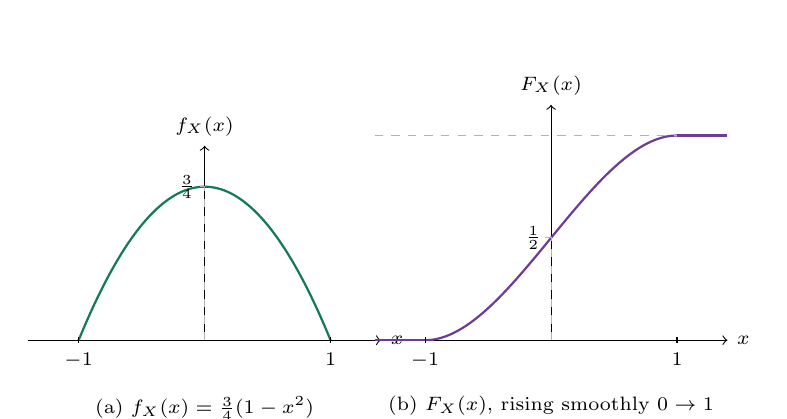
\begin{tikzpicture}[x=1.6cm,y=2.6cm]
\begin{scope}
\draw[->] (-1.4,0) -- (1.4,0) node[right] {\scriptsize $x$};
\draw[->] (0,0) -- (0,0.95) node[above] {\scriptsize $f_X(x)$};
\draw[thmcol,thick,domain=-1:1,smooth,variable=\x,samples=40] plot ({\x},{0.75*(1-\x*\x)});
\draw (-1,-1pt) -- (-1,1pt) node[below=2pt] {\scriptsize $-1$};
\draw (1,-1pt) -- (1,1pt) node[below=2pt] {\scriptsize $1$};
\draw[dashed,gray!60] (0,0) -- (0,0.75) -- (-0.06,0.75);
\node[left] at (0,0.75) {\scriptsize $\frac34$};
\node[below=13pt] at (0,-0.05) {\scriptsize (a) $f_X(x)=\frac34(1-x^2)$};
\end{scope}
\begin{scope}[xshift=4.4cm]
\draw[->] (-1.4,0) -- (1.4,0) node[right] {\scriptsize $x$};
\draw[->] (0,0) -- (0,1.15) node[above] {\scriptsize $F_X(x)$};
\draw[exmcol,thick] (-1.4,0) -- (-1,0);
\draw[exmcol,thick,domain=-1:1,smooth,variable=\x,samples=40] plot ({\x},{0.75*((\x+1)-(1/3)*(\x*\x*\x+1))});
\draw[exmcol,thick] (1,1) -- (1.4,1);
\draw (-1,-1pt) -- (-1,1pt) node[below=2pt] {\scriptsize $-1$};
\draw (1,-1pt) -- (1,1pt) node[below=2pt] {\scriptsize $1$};
\draw[dashed,gray!60] (-1.4,1) -- (1,1);
\draw[dashed,gray!60] (0,0) -- (0,0.5) -- (-0.06,0.5);
\node[left] at (0,0.5) {\scriptsize $\frac12$};
\node[below=13pt] at (0,-0.05) {\scriptsize (b) $F_X(x)$, rising smoothly $0\to1$};
\end{scope}
\end{tikzpicture}
\end{center}

\textit{Step 3 (apply Theorem 4.3/4.1(c)):} $\P{X=0}=0$ (continuous r.v., any single point has
zero probability); $F_X(0)=1/2$; $\P{0<X<0.5}=F_X(0.5)-F_X(0)=11/32$;
$\P{|X-\tfrac12|<\tfrac14}=F_X(3/4)-F_X(1/4)\approx0.2734$.
}

\exambox{Exam 1, Problem 5 --- Gaussian noise, $Q$-function, SNR}{
Definition 4.11 ($Q$-function), Theorem 4.14 (Gaussian CDF via standardizing)}{
Bit-error probability $=\P{X>\sqrt E}=Q(\sqrt{E/\sigma^2})$, SNR$=E/\sigma^2$.

\textit{Step 1 (Theorem 4.14 --- standardize, then Definition 4.11):} with SNR$=4$,
$Q(\sqrt4)=Q(2)=1-\Phi(2)=1-0.97725=\boxed{0.02275}$.

\textit{Step 2 (invert the same relationship):} need $Q(\sqrt{\text{SNR}})<10^{-6}$; from the
$Q$-table this requires $\sqrt{\text{SNR}}\ge4.75\Rightarrow\boxed{\text{SNR}\ge22.56}$.
}

\exambox{Exam 1, Problem 6 (Extra Credit) --- Joint CDF normalizing constant}{
The defining CDF limit $F_{X,Y}(\infty,\infty)=1$ (the 2-D analog of Theorem 4.1(b))}{
$F_{X,Y}(x,y)=a\left[\tfrac\pi2+\tan^{-1}(x/2)\right]\left[\tfrac\pi2+\tan^{-1}(y/3)\right]$.

\textit{Step (take the limit as $x,y\to\infty$ and set it to 1):} since
$\tan^{-1}(\infty)=\pi/2$, each bracket $\to\pi$, so
$\lim F_{X,Y}=a\pi\cdot\pi=1\Rightarrow\boxed{a=1/\pi^2}$. (Checked: as $x,y\to-\infty$ each
bracket $\to0$, so $F(-\infty,y)=F(x,-\infty)=0$ as required of any joint CDF.)
}

\exambox{Exam 1, Problem 7 (Extra Credit) --- Soft limiter, Jacobian method}{
The Chapter 6 general method (\S6.2), applied via the single-variable transformation formula
$f_Y(y)=f_X(x)|dx/dy|$ on each monotonic branch separately}{
$Y=V(1-e^{-X/a})$ for $X\ge0$; $Y=-V(1-e^{X/a})$ for $X\le0$ --- two separate monotonic
branches, so invert each one.

\textit{Step 1 (invert the $X\ge0$ branch):} $y=V(1-e^{-x/a})\Rightarrow
x=a\ln\!\left(\tfrac{V}{V-y}\right)$, giving $dx/dy=a/(V-y)$.

\textit{Step 2 (invert the $X\le0$ branch the same way):} $x=-a\ln\!\left(\tfrac{V}{V+y}\right)$,
giving $dx/dy=a/(V+y)$.

\textit{Step 3 (combine both branches with unit-step indicators $u(y),u(-y)$ to cover the
whole real line):}
\[
f_Y(y)=\frac{a}{V-y}f_X\!\left[a\ln\!\left(\frac{V}{V-y}\right)\right]u(y)+
\frac{a}{V+y}f_X\!\left[-a\ln\!\left(\frac{V}{V+y}\right)\right]u(-y).
\]
}

\clearpage
\section{Exam 2 --- All 5 Problems}

\exambox{Exam 2, Problem 1 --- Joint PDF moments and covariance (textbook 5.7.12)}{
Theorem 5.9 ($\E{XY}$), Theorem 5.16(a) (covariance), Theorem 5.12 (variance of a sum)}{
$f_{X,Y}(x,y)=4xy$ on the unit square.

\textit{Step 1 (Theorem 5.9 --- integrate $x$, $x^2$, $y$, $y^2$, and $xy$ against the joint
PDF):} $\E{X}=\E{Y}=2/3$; $\E{X^2}=\E{Y^2}=1/2\Rightarrow$ (Theorem 4.5(c))
$\Var{X}=\Var{Y}=1/18$; and $\E{XY}=4/9$.

\textit{Step 2 (Theorem 5.16(a) --- $\Cov{X,Y}=\E{XY}-\E{X}\E{Y}$):}
$\Cov{X,Y}=4/9-(2/3)^2=0$.

\textit{Step 3 (Theorem 5.11 then Theorem 5.12):} $\E{X+Y}=4/3$, and since the covariance
term vanishes, $\boxed{\Var{X+Y}=1/18+1/18+2(0)=1/9}$.
}

\exambox{Exam 2, Problem 2 --- Bivariate-Gaussian-type joint PDF (textbook 5.9.5)}{
Definition 5.10 (bivariate Gaussian PDF --- coefficient matching), Theorem 5.19 ($\rho$ is the
correlation coefficient), Theorem 5.20 (uncorrelated $\Leftrightarrow$ independent)}{
$f_{X,Y}(x,y)=ce^{-(2x^2-4xy+4y^2)}$.

\textit{Step 1 (recognize the form and match to Definition 5.10):} write the target exponent
$-\tfrac1{2(1-\rho^2)}\left[\tfrac{x^2}{\sigma_X^2}-\tfrac{2\rho xy}{\sigma_X\sigma_Y}+
\tfrac{y^2}{\sigma_Y^2}\right]$ against $-(2x^2-4xy+4y^2)$ and equate coefficients of
$x^2,xy,y^2$. Since there's no linear term, $\E{X}=\E{Y}=0$.

\textit{Step 2 (solve the coefficient-matching system):} this yields
$\sigma_X=1/\sqrt2,\ \sigma_Y=1/2,\ \boxed{\rho=1/\sqrt2}$.

\textit{Step 3 (Definition 5.10's normalizing constant):}
$c=1/(2\pi\sigma_X\sigma_Y\sqrt{1-\rho^2})=\boxed{2/\pi}$.

\textit{Step 4 (Theorem 5.20):} since $\rho\ne0$ and $X,Y$ are bivariate Gaussian, uncorrelated
would have been equivalent to independent --- but $\rho\ne0$ means \textbf{dependent}.
}

\exambox{Exam 2, Problem 3 --- Power dissipation \& range-limited output (textbook 6.3.10)}{
The $Y=cX^2$ template (Example 6.4/\S6.2), the range-limited/clipped-variable impulse
technique (Examples 6.7--6.8/\S6.3)}{
$X\sim$Uniform$(-2,2)$ (current), $Y=9X^2$ (power, so $c=9$).

\textit{Step 1 (the $F_W\to f_W$ method, \S6.2, with the $Y=cX^2$ clipping refinement):}
$0\le Y<36$; for $0\le y<36$, $F_Y(y)=\P{-\sqrt{y/9}\le X\le\sqrt{y/9}}=\sqrt y/6$ (both
bounds fall inside $X$'s support here, so no clipping is needed) $\Rightarrow$ differentiate:
$f_Y(y)=1/(12\sqrt y)$.

\textit{Step 2 (Examples 6.7--6.8's range-limiting technique --- part (c)):} $W=Y$ if
$Y<16$, else $16$. It helps to first sketch $W$ as a deterministic function of $Y$
(the problem's own suggestion):
\begin{center}
\begin{tikzpicture}[x=0.28cm,y=0.28cm]
\draw[->] (0,0) -- (26,0) node[right] {\scriptsize $y$};
\draw[->] (0,0) -- (0,20) node[above] {\scriptsize $w=g(y)$};
\draw[thmcol,thick] (0,0) -- (16,16);
\draw[thmcol,thick] (16,16) -- (24,16);
\draw[dashed,gray!60] (16,0) -- (16,16) -- (0,16);
\draw (16,-2pt) -- (16,2pt) node[below=2pt] {\scriptsize $16$};
\draw (-2pt,16) -- (2pt,16) node[left=2pt] {\scriptsize $16$};
\end{tikzpicture}
\end{center}
For $0\le w<16$, $F_W(w)=F_Y(w)=\sqrt w/6$ (unchanged, limiter inactive).
At $w=16$ the CDF jumps from $F_Y(16^-)=4/6$ to $1$ --- an impulse of weight
$1-4/6=1/3$ appears in the PDF exactly at the clip point:
$f_W(w)=\tfrac{1}{12\sqrt w}\,(0\le w<16)+\tfrac13\delta(w-16)$.
}

\exambox{Exam 2, Problem 4 --- Joint PDF on a triangle (textbook 5.8.8)}{
Theorem 5.9 ($\E{g(X,Y)}$ for $g=xy$ and $g=e^{x+y}$), Definition 5.7 (correlation)}{
$f_{X,Y}(x,y)=\tfrac12$ on the triangle $-1\le x\le y\le1$.

\textit{Requested sketch of the support region} (shaded), bounded by $x=-1$, $y=1$, and the
line $y=x$:
\begin{center}
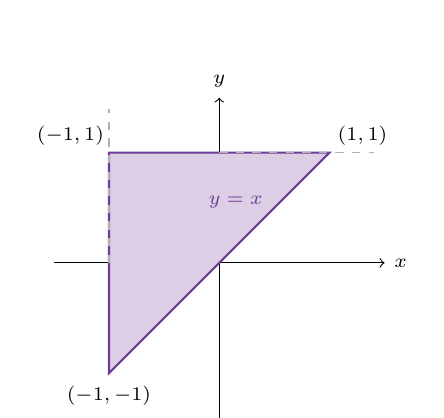
\begin{tikzpicture}[x=1.4cm,y=1.4cm]
\draw[->] (-1.5,0) -- (1.5,0) node[right] {\scriptsize $x$};
\draw[->] (0,-1.5) -- (0,1.5) node[above] {\scriptsize $y$};
\fill[exmcol!25] (-1,-1) -- (-1,1) -- (1,1) -- cycle;
\draw[exmcol,thick] (-1,-1) -- (-1,1) -- (1,1) -- cycle;
\draw[dashed,gray!60] (-1,0) -- (-1,1.4);
\draw[dashed,gray!60] (0,1) -- (1.4,1);
\node at (-1,-1.2) {\scriptsize $(-1,-1)$};
\node at (-1.35,1.15) {\scriptsize $(-1,1)$};
\node at (1.3,1.15) {\scriptsize $(1,1)$};
\node[exmcol] at (0.15,0.55) {\scriptsize $y=x$};
\end{tikzpicture}
\end{center}

\textit{Step 1 (Definition 5.7 via Theorem 5.9 --- integrate $xy$ over the triangle):}
$r_{X,Y}=\E{XY}=\int_{-1}^1\int_x^1\tfrac{xy}2\,dy\,dx=\tfrac14\int_{-1}^1x(1-x^2)dx=\boxed0$
(the integrand is odd in $x$ over a symmetric range).

\textit{Step 2 (Theorem 5.9 again, this time with $g(x,y)=e^{x+y}$):}
$\E{e^{X+Y}}=\int_{-1}^1\int_x^1\tfrac12e^xe^y\,dy\,dx=\tfrac12\int_{-1}^1e^x(e-e^x)dx=
\boxed{e^2/4+e^{-2}/4-1/2}$.
}

\exambox{Exam 2, Problem 5 --- Discrete joint PMF, full moment workup (textbook 5.8.6)}{
Marginal PMF (sum the joint table), Definition 5.7 (correlation), Theorem 5.16(a)
(covariance), Definition 5.6 (correlation coefficient)}{
$P_{X,Y}(x,y)=1/(4x)$ for integers $1\le y\le x\le4$.

\textit{Step 1 (marginalize, then Definition 4.4/Theorem 4.5(c) on each marginal):}
$\E{X}=5/2,\E{Y}=7/4$; $\Var{X}=5/4,\Var{Y}=41/48$.

\textit{Step 2 (Definition 5.7 via Theorem 5.9 --- sum $xy\,P_{X,Y}(x,y)$ over the table):}
$r_{X,Y}=\E{XY}=5$.

\textit{Step 3 (Theorem 5.16(a)):} $\Cov{X,Y}=5-(5/2)(7/4)=10/16$.

\textit{Step 4 (Definition 5.6 --- divide by $\sigma_X\sigma_Y$):}
$\boxed{\rho_{X,Y}=\dfrac{10/16}{\sqrt{(5/4)(41/48)}}\approx0.605}$.
}

\clearpage
\section{Chapter 13 Homework --- All 6 Problems}

\exambox{Problem 13.9.1 --- Which are valid autocorrelation functions?}{
Theorem 13.12 (even, $R(0)\ge|R(\tau)|$), the extra limit property
$\lim_{|\tau|\to\infty}R_X(\tau)=\mu_X^2\ge0$}{
$R_1(\tau)=\delta(\tau)$, $R_2(\tau)=\delta(\tau)+10$, $R_3(\tau)=\delta(\tau-10)$,
$R_4(\tau)=\delta(\tau)-10$.

\textit{Step 1 (Theorem 13.12(b) --- check evenness first, it's the fastest filter):}
$R_1,R_2,R_4$ are all even; $R_3(-\tau)=\delta(\tau+10)\ne R_3(\tau)$ --- \boxed{R_3\text{ is
NOT valid.}}

\textit{Step 2 ($R_1$ --- recognize the white-noise form, Definition 13.20):}
$\delta(\tau)$ is exactly $R_W(\tau)=\eta_0\delta(\tau)$ with $\eta_0=1$. \boxed{\text{Valid.}}

\textit{Step 3 ($R_2$ --- decompose as a sum of two valid ACFs):} $\delta(\tau)+10$ = (white
noise ACF) $+$ (ACF of an independent random-constant process with $\E{A^2}=10$); sums of
independent processes' ACFs are valid ACFs. \boxed{\text{Valid.}}

\textit{Step 4 ($R_4$ --- apply the extra limit property):} even, but
$\lim_{|\tau|\to\infty}R_4(\tau)=-10$, which must equal $\mu_X^2\ge0$ --- contradiction.
\boxed{\text{NOT valid.}}
}

\exambox{Problem 13.9.5 --- Autocorrelation of an iid sequence}{
Definition 13.13 ($R_X[n,k]=\E{X_nX_{n+k}}$), Theorem 4.5(c), Theorem 5.17(b) (independence)}{
$X_n$ iid, $\E{X_n}=\mu$, $\Var{X_n}=\sigma^2$.

\textit{Step 1 ($k=0$, Theorem 4.5(c)):} $R_X[n,0]=\E{X_n^2}=\Var{X_n}+\mu^2=\sigma^2+\mu^2$.

\textit{Step 2 ($k\ne0$, independence + Theorem 5.17(b)):} $X_n,X_{n+k}$ are independent
$\Rightarrow R_X[n,k]=\E{X_n}\E{X_{n+k}}=\mu^2$.

\[ \boxed{R_X[n,k] = \begin{cases}\sigma^2+\mu^2 & k=0\\ \mu^2 & k\ne0\end{cases}} \]
}

\exambox{Problem 13.9.9 --- WSS process times a random-phase cosine}{
Definition 13.16 (average power), Example 13.22's lemma, Theorem 5.17(a) (independence)}{
$X(t)$ WSS, $R_X(0)=\E{X^2(t)}=1$; $\Theta\sim$Uniform$(0,2\pi)$ independent of $X(t)$.

\textit{(a) Definition 13.16 directly:} $\E{X^2(t)}=R_X(0)=\boxed1$.

\textit{(b) Example 13.22's lemma with $a=2\pi f_ct,k=1$:} $\E{\cos(2\pi f_ct+\Theta)}=
\boxed0$.

\textit{(c) Theorem 5.17(a) on $Y(t)=X(t)\cos(2\pi f_ct+\Theta)$:}
$\E{Y(t)}=\E{X(t)}\cdot\E{\cos(2\pi f_ct+\Theta)}=\E{X(t)}\cdot0=\boxed0$.

\textit{(d) Theorem 5.17(a) again, then the lemma with $k=2$:}
$\E{Y^2(t)}=\E{X^2(t)}\cdot\E{\cos^2(2\pi f_ct+\Theta)}=1\cdot\left[\tfrac12+\tfrac12\E{\cos(4\pi f_ct+2\Theta)}\right]=1\cdot\tfrac12=\boxed{1/2}$.
}

\exambox{Problem 13.10.1 --- Product of two independent WSS processes}{
The product-of-independent-WSS-processes technique (this page's flagged entry above),
Theorem 5.17(a)}{
$X(t),Y(t)$ independent WSS, means $\mu_X,\mu_Y$, autocorrelations $R_X(\tau),R_Y(\tau)$;
$W(t)=X(t)Y(t)$.

\textit{(a) Mean and autocorrelation, via independence:} $\mu_W=\mu_X\mu_Y$;
$R_W(t,\tau)=\E{X(t)X(t+\tau)}\cdot\E{Y(t)Y(t+\tau)}=R_X(\tau)R_Y(\tau)$ --- $\tau$-only
$\Rightarrow\boxed{W(t)\text{ is WSS.}}$

\textit{(b) Cross-correlation with $X(t)$:}
$R_{WX}(t,\tau)=\E{X(t)X(t+\tau)}\cdot\E{Y(t)}=R_X(\tau)\mu_Y$ --- $\tau$-only
$\Rightarrow\boxed{\text{yes, jointly WSS.}}$
}

\exambox{Problem 13.10.3 --- Autocorrelation/cross-correlation of a delayed process}{
Definition 13.13 (autocorrelation), Definition 13.17/13.18 (cross-correlation, jointly WSS)}{
$X(t)$ WSS, $R_X(\tau)=10\sin(2000\pi\tau)/(2000\pi\tau)$; $Y(t)=X(t-t_0)$,
$t_0=5\times10^{-5}$s.

\textit{(a) The two arguments of $X$ differ by $\tau$ regardless of $t_0$:}
$\boxed{R_Y(\tau)=R_X(\tau)}$ --- delaying a WSS process doesn't change its ACF.

\textit{(b) The two arguments now differ by $\tau-t_0$:}
$\boxed{R_{XY}(\tau)=R_X(\tau-t_0)}$.

\textit{(c)} $R_Y(\tau)$ depends on $\tau$ only and $\mu_Y=\mu_X$ (constant)
$\Rightarrow\boxed{Y(t)\text{ is WSS.}}$

\textit{(d)} $R_{XY}(t,\tau)=R_X(\tau-t_0)$ depends on $\tau$ only
$\Rightarrow\boxed{\text{jointly WSS.}}$
}

\exambox{Problem 13.11.2 --- Which transforms of a Gaussian process stay Gaussian?}{
Definition 13.19 (Gaussian process), Theorem 5.21/8.11 (linear transforms of Gaussian
vectors are Gaussian)}{
Given Gaussian $X(t)$: (a) $2X(t)$, (b) $X(t/2)$, (c) $X(t)/2$, (d) $X(t)-X(t-1)$,
(e) $X(2t)$.

\textit{Step 1 (scalar multiples, (a) and (c)):} $[2X(t_1),\dots,2X(t_k)]'$ and
$[X(t_1)/2,\dots,X(t_k)/2]'$ are linear (scalar) transforms of a Gaussian vector.
\boxed{\text{Gaussian.}}

\textit{Step 2 (time re-indexing, (b) and (e)):} $[X(t_1/2),\dots,X(t_k/2)]'$ and
$[X(2t_1),\dots,X(2t_k)]'$ are just samples of $X$ at different (still arbitrary) time
instants --- Gaussian by Definition 13.19 directly. \boxed{\text{Gaussian.}}

\textit{Step 3 (linear combination across two times, (d)):}
$[X(t_1)-X(t_1-1),\dots,X(t_k)-X(t_k-1)]'$ is a linear transform of the $2k$-dimensional
Gaussian vector $[X(t_1),X(t_1-1),\dots,X(t_k),X(t_k-1)]'$. \boxed{\text{Gaussian.}}

\boxed{\text{All five (a)--(e) are Gaussian processes.}}
}

\clearpage
% ================================================================
\section*{One-Page Recap: How Each Exam Problem Is Solved --- Theorem \& Technique at a Glance}
\addcontentsline{toc}{section}{One-Page Recap}

\noindent This table is the theoretical skeleton behind every solution in
Part~\ref{part:exams}: for each problem, \emph{which theorem} supplies the formula and
\emph{which technique} turns that formula into the answer. Study this table first --- it is
the pattern you are expected to reproduce on the final for a similarly-worded question.

{\small
\begin{longtable}{@{}p{2.5cm}p{4.7cm}p{6.4cm}@{}}
\toprule
\textbf{Problem} & \textbf{Theorem(s) used} & \textbf{Technique --- \emph{how} it's solved}\\
\midrule
\endhead
Exam 1, P1 (mixed r.v.) & Def.\ 4.12, Thm.\ 4.16, Thm.\ 4.2, Thm.\ 4.1(c)/4.17 &
\textbf{Normalize-then-integrate:} impulse probabilities are fixed numbers, so subtract their
total from 1 to get the continuous part's required area; solve for the constant. Then build
$F_X$ by integrating the continuous density piecewise and adding each impulse's full weight as
a jump the instant $x$ crosses it.\\[4pt]
Exam 1, P2 (joint PDF $\to$ marginal $\to$ moments) & Marginalization, Thm.\ 4.4 (LOTUS),
Thm.\ 4.5(c) & \textbf{Reduce to one variable:} integrate the joint PDF over the \emph{other}
variable to get $f_X(x)$ alone, then solve it as an ordinary single-variable problem
($\E{X}$, $\E{X^2}$, subtract the square for variance).\\[4pt]
Exam 1, P3 (joint PMF table) & Marginal PMF (row/column sums), Def.\ 4.4, Thm.\ 4.5(c) &
\textbf{Sum the table:} row sums give one marginal, column sums the other; event probabilities
are sums of the specific cells satisfying the event; moments follow from the marginal exactly
as in the continuous case, just with sums instead of integrals.\\[4pt]
Exam 1, P4 (normalize a PDF) & Thm.\ 4.2, Thm.\ 4.1/4.3 & \textbf{Set $\int f_X=1$} and solve
for the constant; integrate once more to get $F_X$; every subsequent probability is then a
plug-in evaluation or difference of $F_X$.\\[4pt]
Exam 1, P5 (Gaussian/$Q$-function/SNR) & Def.\ 4.11, Thm.\ 4.14 & \textbf{Standardize, then
table-lookup:} rewrite the event in terms of $Q(z)$ or $\Phi(z)$ with $z$ a function of the
given parameter (here $\sqrt{\text{SNR}}$); to go the other direction (part (b)), invert the
$Q$-table to find the $z$ that achieves the target probability.\\[4pt]
Exam 1, P6 (joint CDF constant) & $F_{X,Y}(\infty,\infty)=1$ & \textbf{Take the defining
limit:} let $x,y\to\infty$ in the given formula (using known limits like $\tan^{-1}(\infty)$),
set the result equal to 1, and solve for the constant.\\[4pt]
Exam 1, P7 (soft limiter) & Ch.\ 6 general method, $f_Y=f_X|dx/dy|$ & \textbf{Invert each
monotonic branch separately:} split the domain where $g$ is monotonic, solve $y=g(x)$ for $x$
on each piece, multiply $f_X$ at that $x$ by $|dx/dy|$, and stitch the pieces together with
unit-step indicators.\\[4pt]
Exam 2, P1 (joint PDF moments/covariance) & Thm.\ 5.9, Thm.\ 5.16(a), Thm.\ 5.12 &
\textbf{Moments first, combine second:} compute $\E{X},\E{Y},\E{X^2},\E{Y^2},\E{XY}$ all by
direct double integration (Thm.\ 5.9), then get $\Cov{X,Y}$ and $\Var{X+Y}$ purely
algebraically from those numbers --- never integrate $(x-\mu_X)(y-\mu_Y)$ directly.\\[4pt]
Exam 2, P2 (bivariate-Gaussian-type PDF) & Def.\ 5.10, Thm.\ 5.19, Thm.\ 5.20 &
\textbf{Coefficient matching:} recognize the $ce^{-(\text{quadratic})}$ form, equate its
quadratic's coefficients term-by-term with Definition 5.10's exponent to solve for
$\sigma_X,\sigma_Y,\rho$ simultaneously, then get $c$ from the normalizing constant; use
$\rho\ne0$ to conclude dependence via Theorem 5.20.\\[4pt]
Exam 2, P3 (power dissipation, range-limited) & $Y=cX^2$ template (Ex.\ 6.4), clip-impulse
technique (Ex.\ 6.7--6.8) & \textbf{Two-stage transform:} first derive $F_Y$ by translating
$\{Y\le y\}$ into a symmetric interval on $X$ and integrating (clipping to $X$'s support if
needed); then, for the range-limited version, keep $f_Y$ unchanged below the clip and add an
impulse at the clip point weighted by the clipped-away tail probability.\\[4pt]
Exam 2, P4 (joint PDF on a triangle) & Thm.\ 5.9, Def.\ 5.7 & \textbf{Set up the double
integral over the triangular support} (inner limit depends on the outer variable), then
evaluate directly for whichever function $g(x,y)$ ($xy$, or $e^{x+y}$) is asked for.\\[4pt]
Exam 2, P5 (discrete joint PMF workup) & Marginal PMF, Def.\ 5.7, Thm.\ 5.16(a), Def.\ 5.6 &
\textbf{Same pipeline as P1, discrete version:} marginalize by summing the table, get
$\E{XY}$ by summing $xy\,P_{X,Y}(x,y)$ over all cells, then chain into covariance and
$\rho_{X,Y}$ algebraically.\\[4pt]
HW 13.9.1 (valid ACF?) & Thm.\ 13.12, limit property $\lim_{|\tau|\to\infty}R_X(\tau)=\mu_X^2$
& \textbf{Test each candidate against Theorem 13.12:} check evenness first (fastest
rejection), then $R(0)\ge|R(\tau)|$, then the limit-as-$|\tau|\to\infty$ property; a
candidate that's a sum of two individually-valid ACFs is itself valid.\\[4pt]
HW 13.9.5 ($R_X[n,k]$ of an iid sequence) & Def.\ 13.13, Thm.\ 4.5(c), Thm.\ 5.17(b) &
\textbf{Split on $k=0$ vs.\ $k\ne0$:} at $k=0$ use $\E{X_n^2}=\Var{X_n}+\mu^2$; at $k\ne0$ use
independence to factor $\E{X_nX_{n+k}}=\E{X_n}\E{X_{n+k}}$.\\[4pt]
HW 13.9.9 (WSS process $\times$ random-phase cosine) & Def.\ 13.16, Example 13.22's lemma,
Thm.\ 5.17(a) & \textbf{Factor every expectation using independence} of $X(t)$ and $\Theta$,
then apply Example 13.22's $\E{\cos(a+k\Theta)}=0$ lemma to kill the oscillating terms.\\[4pt]
HW 13.10.1 (product of independent WSS processes) & The product-of-independent-processes
technique, Thm.\ 5.17(a) & \textbf{Split $\E{W(t)W(t+\tau)}$ into
$\E{X(t)X(t+\tau)}\cdot\E{Y(t)Y(t+\tau)}=R_X(\tau)R_Y(\tau)$} using independence of the two
processes --- multiply autocorrelations instead of adding them (contrast with the
signal-plus-noise \emph{sum} template).\\[4pt]
HW 13.10.3 (delayed process, cross-correlation) & Def.\ 13.13, Def.\ 13.17/13.18 &
\textbf{Track the time difference between the two arguments of $X$:} for $R_Y$ it stays
$\tau$ (delay cancels); for $R_{XY}$ it becomes $\tau-t_0$ --- read the answer straight off
$R_X$ evaluated at that difference.\\[4pt]
HW 13.11.2 (Gaussian process under transforms) & Def.\ 13.19, Thm.\ 5.21/8.11 & \textbf{Two
closure facts do all five parts:} scalar multiples and linear combinations of Gaussian
samples stay Gaussian (Thm.\ 5.21/8.11), and re-indexing time (even nonlinearly, e.g.\
$t\mapsto2t$) still just samples $X$ at particular instants (Def.\ 13.19).\\
\bottomrule
\end{longtable}
}

\section*{Exam Pattern Analysis: What the Professor Actually Tests, in Plain Language}
\addcontentsline{toc}{section}{Exam Pattern Analysis}

\noindent Every problem from Exam 1, Exam 2, and the Chapter 13 homework was sorted below into
one of nine ``types.'' For each type you get: how often it showed up, what you're really being
asked to do (in plain words), and the steps --- with the actual numbers from a real problem
attached to each step, so you can see exactly how the idea turns into an answer.

\begin{center}
\fcolorbox{flagcol}{flagbg}{\parbox{\dimexpr\linewidth-2\fboxsep-2\fboxrule}{\centering
\textbf{\color{flagcol}The Headline Finding}\\[4pt]
Of the \textbf{12} Chapter 4--6 exam problems, \textbf{5 (42\%)} are all the same underlying
task: boil a two-variable problem down to a few plain numbers, then combine those numbers with
simple arithmetic (Type 2 below) --- by far the most-repeated skill on both exams. Of the
\textbf{6} Chapter 13 homework problems, \textbf{3 (50\%)} are all about splitting an average
because two things don't affect each other (Type 8 below). \textbf{If you only have time to
practice two things before the final, practice these two.}
}}
\end{center}

\subsection*{Chapters 4--6: Six Problem Types (from Exam 1 \& Exam 2)}

\cheat{Type 1 --- Solve for the Missing Number, Then Build the Full Probability Curve}{
\textbf{Seen in:} Exam 1, Problems 1 and 4 \quad (2 of 12)
}{
You're given a probability curve --- the PDF, $f_X(x)$ --- with one unknown number sitting in
it. Pin down that number first, then use it to write out the complete ``chance $X$ is at most
$x$'' curve, the CDF, $F_X(x)$.
}{
\textbf{Walked through using Exam 1, Problem 1} (three separate spots of guaranteed
probability, plus a smooth curve in between): \textbf{Step 1 --- add up what's already
accounted for.} The three fixed spots already total $\tfrac18+\tfrac1{16}+\tfrac1{16}=\tfrac14$
of all the probability. \textbf{Step 2 --- the rest has to come from the smooth part.} Every
PDF must satisfy $\int f_X(x)\,dx=1$, so set the smooth part's area equal to what's left over
($\tfrac34$) and solve --- this gives the missing number, $A=9/64$. \textbf{Step 3 --- build
the curve piece by piece.} $F_X(x)=\int f_X$: add up the smooth part as you go, and every time
you pass one of the three fixed spots, jump up by that spot's full amount. \textbf{Step 4 ---
answer the actual question.} Read $F_X$ at the value you need straight off the curve you just
built (or subtract two values of $F_X$).
}

\cheatflag{Type 2 --- Boil a Two-Variable Problem Down to a Few Numbers}{
\textbf{Seen in:} Exam 1, Problems 2 and 3; Exam 2, Problems 1, 4, and 5 \quad (5 of 12 ---
\textbf{the most common type by far})
}{
You're given a rule connecting two variables, but the question only asks for averages
($\E{X}$), spread ($\Var{X}$), or how the two move together ($\Cov{X,Y}$). You don't need to
solve the whole two-variable puzzle --- just boil it down to a handful of plain numbers and
combine them with simple arithmetic.
}{
\textbf{Walked through using Exam 2, Problem 1} (the rule $f(x,y)=4xy$ on the unit square):
\textbf{Step 1 --- get each variable on its own, if needed.} Add up (or integrate over) the
other variable to get one variable's own curve, $f_X(x)$ (this is called the \emph{marginal}).
(Not even needed here, since the plain averages below can be read straight off the
two-variable rule.) \textbf{Step 2 --- compute the plain averages.} The average of $X$
($\E{X}$), the average of $Y$ ($\E{Y}$), the average of $X^2$ ($\E{X^2}$), and the average of
$X$ times $Y$ ($\E{XY}$), each found by direct calculation: $\E{X}=2/3$, $\E{X^2}=1/2$,
$\E{XY}=4/9$. \textbf{Step 3 --- combine with simple formulas.} Spread of $X$
($\Var{X}$) $=\E{X^2}-(\E{X})^2=1/2-(2/3)^2=1/18$. How $X$ and $Y$ move together
($\Cov{X,Y}$) $=\E{XY}-\E{X}\E{Y}=4/9-(2/3)^2=0$. \textbf{Step 4 --- combine further if
asked.} Spread of $X+Y$ ($\Var{X+Y}$) $=\Var{X}+\Var{Y}+2\Cov{X,Y}=1/18+1/18+2(0)=1/9$.
}

\cheat{Type 3 --- Matching a Two-Variable Bell-Curve Formula}{
\textbf{Seen in:} Exam 2, Problem 2 \quad (1 of 12, but this exact style is one of the
professor's personal must-knows --- treat it as very likely to reappear)
}{
You're handed a two-variable, bell-curve-shaped formula with an unknown front constant and
some unknown ``spread'' ($\sigma_X,\sigma_Y$) and ``how-they-relate'' ($\rho_{X,Y}$) numbers
hidden inside it. Line it up against the standard bell-curve formula, piece by piece, to read
those numbers off.
}{
\textbf{Walked through using Exam 2, Problem 2} (the rule $ce^{-(2x^2-4xy+4y^2)}$):
\textbf{Step 1 --- recognize the shape.} A constant times ``$e$'' to a negative quadratic in
$x$ and $y$ --- here the quadratic is $2x^2-4xy+4y^2$. \textbf{Step 2 --- line it up against
the standard formula.} The standard two-variable bell curve has known slots for $\sigma_X$,
$\sigma_Y$, and $\rho_{X,Y}$; matching term by term gives $\sigma_X=1/\sqrt2$,
$\sigma_Y=1/2$, $\rho_{X,Y}=1/\sqrt2$. \textbf{Step 3 --- get the front constant.} Plug those
three numbers into the standard formula's constant to get $c=2/\pi$. \textbf{Step 4 --- state
the conclusion.} Since $\rho_{X,Y}$ isn't zero, the two variables are \emph{not} independent
--- knowing one tells you something real about the other.
}

\cheatflag{Type 4 --- Turning One Random Variable Into Another}{
\textbf{Seen in:} Exam 1, Problem 7; Exam 2, Problem 3 \quad (2 of 12 --- consistently the
hardest, last problem on each exam)
}{
You're given a rule for building a new variable $W=g(X)$ out of an old one (e.g.\ squaring it,
or running it through some circuit), and asked for the \emph{whole probability curve} of the
new variable, $f_W(w)$ --- not just its average.
}{
\textbf{Walked through using Exam 2, Problem 3} ($X$ is the current, evenly spread between
$-2$ and $2$; $Y=9X^2$ is the power): \textbf{Step 1 --- figure out what values the new
variable can take.} Since $X$ is between $-2$ and $2$, $Y=9X^2$ can only land between $0$ and
$36$. \textbf{Step 2 --- rewrite ``$Y$ at most $y$'' ($F_Y(y)$) as a statement about the old
variable.} ``$Y\le y$'' means ``$X$ is between $-\sqrt{y/9}$ and $\sqrt{y/9}$''; since $X$ is
evenly spread, that chance is just (length of that stretch)/(total length), giving
$F_Y(y)=\sqrt y/6$. \textbf{Step 3 --- watch the edges.} If those square-root bounds ever stick
out past where the old variable is actually allowed to be, stop them at its edge instead
(didn't happen here, but often does --- check every time). \textbf{Step 4 --- take the
derivative.} $f_Y(y)=dF_Y/dy$ turns $\sqrt y/6$ into the final answer, $1/(12\sqrt y)$.
\textbf{Step 5 --- if the problem then caps the new variable at some value} (like a meter that
can't read above $16$), the curve $f$ stays the same below the cap, and one extra pile of
leftover probability (size $1-4/6=1/3$ here) sits right at the cap.
}

\cheat{Type 5 --- Bell-Curve Probabilities Way Out in the Tail}{
\textbf{Seen in:} Exam 1, Problem 5 \quad (1 of 12)
}{
Ordinary bell-curve (Gaussian) random variable, but the question asks about something rare or
far from the average --- like an error rate.
}{
\textbf{Walked through using Exam 1, Problem 5} (bit-error rate vs.\ signal strength):
\textbf{Step 1 --- rescale to ``how many spreads from the average''} ($z=(x-\mu)/\sigma$).
Subtract the average $\mu$, divide by the spread $\sigma$. \textbf{Step 2 --- use the far-tail
table ($Q$), not the middle-of-the-curve one ($\Phi$),} whenever the question is about
something rare (``chance of error''). With signal strength $4$, this gives
$Q(2)\approx0.0228$. \textbf{Step 3 --- if the question runs backward} (``how strong must the
signal be so the error rate is under one in a million?''), look up the $Q$-table
\emph{backward} to find the cutoff point $z$ first ($4.75$), then solve for the original
quantity (signal strength must be at least $22.56$).
}

\cheat{Type 6 --- Using the Far Edges of a Two-Variable Curve to Find a Constant}{
\textbf{Seen in:} Exam 1, Problem 6 (extra credit) \quad (1 of 12)
}{
You're given a two-variable ``chance both are at most these values'' formula
($F_{X,Y}(x,y)$) with an unknown constant, and told that way out at the far edges, the total
chance must reach exactly $1$: $F_{X,Y}(\infty,\infty)=1$.
}{
\textbf{Walked through using Exam 1, Problem 6:} \textbf{Step 1 --- push both variables out to
plus-infinity} in the given formula and simplify (here, using that an arctangent approaches a
known fixed value far out). \textbf{Step 2 --- set that equal to $1$ and solve} for the
constant, giving $a=1/\pi^2$. \textbf{Step 3 --- sanity-check the other edges}: push the
variables to minus-infinity instead and confirm you get $0$, as any such formula must
($F_{X,Y}(-\infty,y)=0$).
}

\subsection*{Chapter 13: Three Problem Types (from the Homework Set)}

\cheat{Type 7 --- Checking Whether a Formula Could Really Describe a Self-Correlation}{
\textbf{Seen in:} Homework 13.9.1 \quad (1 of 6, but tests the professor's personally-flagged
theorem --- treat it as very likely to reappear)
}{
You're handed a candidate formula and asked whether it's even \emph{allowed} to be an
autocorrelation, written $R_X(\tau)$ or $R(\tau)$ --- a measure of how a signal lines up with a
delayed copy of itself, $\tau$ seconds later.
}{
\textbf{Walked through using Homework 13.9.1} (four candidate formulas for $R(\tau)$):
\textbf{Step 1 --- check that flipping the sign of the delay doesn't change the answer:}
$R(\tau)$ must equal $R(-\tau)$. One candidate here failed immediately: shifting a spike to
$\tau=+10$ instead of $\tau=-10$ gave a different formula. \textbf{Step 2 --- check that
$R(0)$ (``no delay at all'') is the single biggest value} the formula ever reaches:
$R(0)\ge|R(\tau)|$. \textbf{Step 3 --- check that, far away, $R(\tau)$ settles down to
something zero or positive --- never negative} ($\lim_{|\tau|\to\infty}R(\tau)\ge0$). One
candidate here settled down to $-10$, which is impossible, so it was ruled out too.
}

\cheatflag{Type 8 --- Splitting an Average When Two Things Don't Affect Each Other}{
\textbf{Seen in:} Homework 13.9.5, 13.9.9, and 13.10.1 \quad (3 of 6 --- \textbf{the single
most common Chapter 13 skill})
}{
You need the average of a product of two things ($\E{AB}$), and those two things have no
effect on each other at all (they're \emph{independent}) --- so you're allowed to average each
one separately and just multiply the results: $\E{AB}=\E{A}\E{B}$.
}{
\textbf{Walked through using Homework 13.10.1} (two completely separate signals $X(t),Y(t)$
multiplied together, $W(t)=X(t)Y(t)$): \textbf{Step 1 --- confirm exactly what doesn't affect
what.} Here, the two whole signals are unrelated to each other. \textbf{Step 2 --- split the
average of the product into a product of averages.} The autocorrelation of $W$,
$R_W(\tau)=\E{W(t)W(t+\tau)}=\E{X(t)X(t+\tau)}\cdot\E{Y(t)Y(t+\tau)}=R_X(\tau)R_Y(\tau)$ ---
signal 1's own self-correlation times signal 2's own self-correlation. \textbf{Step 3 ---
watch for a special case.} Sometimes ``no delay'' ($\tau=0$, or $k=0$ for a sequence) behaves
differently from ``some delay,'' or a spinning random angle averages away to exactly zero ---
handle that piece on its own when it comes up. \textbf{Step 4 --- put the pieces back
together} to get the final formula.
}

\cheat{Type 9 --- Following a Time-Shift Through the Formula}{
\textbf{Seen in:} Homework 13.10.3 and 13.11.2 \quad (2 of 6)
}{
A new signal is built by delaying, speeding up/slowing down, or combining samples of an old
one. Track exactly which time-gap ends up mattering inside $R_X(\cdot)$, or confirm the new
signal is still bell-curve-shaped (Gaussian) if the old one was.
}{
\textbf{Walked through using Homework 13.10.3} (a plain delayed copy of a signal,
$Y(t)=X(t-t_0)$): \textbf{Step 1 --- write down the two specific time points being compared}
(for $R_Y(\tau)=\E{Y(t)Y(t+\tau)}$, that's $t-t_0$ and $t+\tau-t_0$). \textbf{Step 2 ---
subtract them to get the time-gap that actually matters:} here it's just $\tau$ again. A pure
delay applied to \emph{both} copies leaves this gap --- and so $R_X(\cdot)$ --- completely
unchanged: $R_Y(\tau)=R_X(\tau)$. Comparing the original to a delayed copy instead
($R_{XY}(\tau)=\E{X(t)Y(t+\tau)}$) shifts the gap by however long the delay is:
$R_{XY}(\tau)=R_X(\tau-t_0)$. \textit{(A related question, Homework 13.11.2, asks about
combining or re-timing a Gaussian signal instead: doubling it, subtracting two of its samples,
or sampling it at different times never breaks the ``still Gaussian'' property --- that part
is automatic.)}
}

\subsection*{If a Final-Exam Question Doesn't Match Any of These Nine Exactly}
It's almost certainly a small variation on one of them. Ask yourself: is this a
one-variable-curve question (Type 1)? A two-variable-averages question (Type 2 --- the most
likely by far)? A bell-curve-formula-matching question (Type 3)? A build-a-new-variable
question (Type 4)? A far-tail bell-curve question (Type 5)? A find-the-constant-from-the-edges
question (Type 6)? For Chapter 13: a check-the-formula question (Type 7)? A
split-the-average question (Type 8 --- the most likely of the three)? Or a
follow-the-time-shift question (Type 9)? Once you know which one it is, the steps above tell
you exactly what to do.

\finalline{flagcol}
\begin{center}
\textit{Companion document: \texttt{Final\_Exam\_Guide.pdf} --- full proofs, complete worked
examples, and every Exam 1 / Exam 2 problem solved step by step.}
\end{center}

\end{document}
